%%%%%%%%%%%%%%%%%%%%%%%%%%%%%%%%%%%%%%%%%%%
%
% szablon pracy licencjackiej 
% korzystający ze stylu pracalicmgr.cls
% 2017.03.22 K. Turzynski
% 2017.03.01 P. Durka durka@fuw.edu.pl 
% na podstawie pliku J. Żygierewicz 2016
%
%%%%%%%%%%%%%%%%%%%%%%%%%%%%%%%%%%%%%%%%%%%

\documentclass{pracalicmgr}
\usepackage{array}
\usepackage{graphicx}
\usepackage{multirow}
\usepackage{amssymb}
\usepackage{graphics}
\usepackage{mathtools}
\usepackage{hyperref}
\usepackage{amsmath}
\usepackage{subcaption}
\DeclareMathOperator{\Var}{\widehat{Var}}
\usepackage{url}
\usepackage{float}
\usepackage{physics}
\usepackage{natbib}
\usepackage[utf8x]{inputenc}
\usepackage[T1]{fontenc}
\usepackage[english]{babel}
\usepackage[nottoc]{tocbibind}
\usepackage{lipsum}  
\usepackage{courier}
\usepackage[toc,page]{appendix}
\usepackage{changepage}
\usepackage{wrapfig}
\newcommand{\summary}[1]{
    \begin{center}
        \Huge #1
    \end{center}
    \begin{figure}[H]
        \centering
        \begin{adjustwidth}{-0.5in}{-0.5in}
        \begin{subfigure}{0.6\textwidth}
            \centering
            \includegraphics[width=1\textwidth]{plots/#1_phase.png}
            \caption{The phased light curve in the I band using OGLE data.}
        \end{subfigure}
        %\hfill
        \begin{subfigure}{0.6\textwidth}
            \centering
            \includegraphics[width=1\textwidth]{plots/#1_simple_corner_emcee.png}
            \caption{Corner plot for the posterior estimate of SED.}
        \end{subfigure}
        \end{adjustwidth}
   \end{figure}
    \begin{figure}[H]
        \centering
        \begin{adjustwidth}{-0.5in}{-0.5in}
        \begin{subfigure}{0.6\textwidth}
            \centering
            \includegraphics[width=1\textwidth]{plots/#1_simple_emcee.png}
            \caption{The spectral energy distribution plot for the single star model.}
        \end{subfigure}
        %\hfill
        \begin{subfigure}{0.6\textwidth}
            \centering
            \includegraphics[width=1\textwidth]{plots/#1_HR.png}
            \caption{Position in HR diagram together with the best-fitting PARSEC evolutionary track.}
        \end{subfigure}
        \end{adjustwidth}
   \end{figure}
   \newpage
}

\newenvironment{itemize*}%
  {\vspace{-\topsep}
    \begin{itemize}%
    \setlength{\itemsep}{0pt}%
    \setlength{\parskip}{0pt}}%
  {\end{itemize}
  \vspace{-\topsep}}


\author{Mateusz Kapusta}


\nralbumu{431289}

\title{Search for Dormant Black Holes in OGLE data.}

\tytulang{Poszukiwanie uśpionych czarnych dziur w danych z przeglądu OGLE.}

\kierunek{studiów fizyka}

%\specjalnosc{$<$Specjalność-o-ile-dotyczy$>$}

\opiekun{dr Przemysław Mróz \\Astronomical Observatory\\Warsaw University}

%\dziedzina{13.200}
%\dziedzina{13.2 Fizyka}

\date{May 2023}

\keywords{Compact Objects, Ellipsoidal variables}



\begin{document}
    \maketitle
    \let\cleardoublepage\clearpage
\begin{abstract}
    In the work analysis of light curves from OGLE data was performed with the goal to look for objects with possible black hole companions 
    based on the ellipsoidal modulation of light curves. Each object is examined using the spectral energy distribution fit, allowing one to distinguish
    between stars composed of two objects with different temperatures and single objects. The selection process resulted in fourteen
    potential objects out of which one turned out to be the spotted star, while the rest are considered black hole binaries candidates.
    Detailed analysis of objects is conducted estimating basic physical parameters such as temperature, mass, radius,
    and, in some cases, estimate of radial velocity. Although in the end an alternative explanation for ellipsoidal modulation is given, 
    no conclusion is reached as objects should be further observed spectroscopically to accept or reject the hypothesis about compact companions.
\end{abstract}

\tableofcontents

\chapter{Introduction}
According to the current knowledge, O type stars (which are more massive than $20$ M$_\odot$) end their evolution as black holes, further investigation suggests
the existence of $\mathcal{O}(10^8)$ stellar mass BHs \citep{brown_scenario_1994} in our Galaxy.
Despite a huge theoretical expectation, only a few tens of such objects have been found up to day.
Since the discovery of the first black hole binary Cygnus X-1 many researchers have tried to tackle the problem employing numerous methods with particular
success achieved in the field of X-ray based observations. Although such observations can be a great tool for black hole search, there are quite limited,
as formation of such systems is rare \citep{zwart_formation_1997}. Since the beginning of LIGO/VIRGO observations of merging black holes,
interest in the progenitors of black hole merger events began to grow. Despite many surveys and theoretical works, 
no conclusions were reached about formation mechanisms for many black hole mergers. 

The vast majority of black hole binaries were discovered due to X-ray emission from an accreation disc that is forming in a system.
X-ray emitting objects can be roughly grouped into two categories: low-mass X-ray binaries and high-mass X-ray binaries (referred to as LMXB and HMXB).
Low-mass binaries are composed of a compact object that is accreting matter from a low-mass companion overflowing its Roche lobe. On the other hand, high-mass X-ray
binaries accreate matter from a stellar wind created by a high-mass companion star.
The X-ray emission from the X-ray binaries is mostly transient in character \citep{bambi_transient_2016}
due to the instability of the accretion disc \citep{lasota_disc_2001}. Many of the X-ray binaries can remain undetected in the low-accreating
regime for long periods, hence an all-sky monitoring in X-rays is necessary. According to \citet{corral-santana_blackcat_2016} 
only $64$ stellar BH X-ray binaries have been detected to the present day, while only $5$ of them are considered persistent sources. 
Of all those sources, only around $\sim 20$ of them are dynamically confirmed (from dynamically confirmed binaries only Cygnus X-1 is persistent). 
The rest of the candidates were not observed spectroscopically, as they are faint in quiescence, distant, or lie in high-extinction regions. 
Although most of the observed BH binaries emit X-rays such systems should be outnumbered by nonaccreating binaries \citep{langer_properties_2020}. 
The estimated total number of X-ray black holes in the Milky Way is around $\sim 10^3$ \citep{corral-santana_blackcat_2016}, suggesting that only small fraction
of such systems was discovered. It is hard to determine how many of those binaries can be detected as search for such transient objects can be problematic.
Nevertheless, both theoretical and observational arguments agree that that potential population of black hole X-ray binaries is rather limited.

In recent years new stellar mass BH candidates have been found due to the new methods not based on X-ray emission. New generations of sky surveys
including spectroscopic surveys like APOGEE, LAMOST and GALAH can provide radial velocity information for millions of stars. Such
information itself can be used to search for compact objects and there are numerous candidates for compact binaries that are dormant in the
X-ray including black hole binaries (\citet{liu_wide_2019}, \citet{jayasinghe_asas-sn_2019}, \citet{shenar_x-ray-quiet_2022}, \citet{lennon_vlt-flames_2022},
\citet{thompson_noninteracting_2019}).
Although many of those claims have been disputed,
one can expect such surveys to provide an increasing number of potential black hole binaries. Unfortunately, even wide-field multi-fibre spectroscopic
devices cannot observe as many objects at once as wide-field photometric devices, limiting the size of the sample that can be studied with this type of
survey. There are also new discoveries of potential black hole binaries using Gaia astrometric observations coupled with spectroscopic follow-up 
observations \citep{el-badry_sun-like_2022,el-badry_red_2023}.
Binaries with sufficiently long periods
paired with low parallaxes allow one to resolve components of binary and trace apparent movement on the sky.
This type of observation is available only for a relatively small sample of objects ($\sim 30000$) at the moment,
but with the next releases of Gaia data, this number is expected to increase significantly. Astrometric observations
are powerful and on their own enable one to estimate masses of objects via the astrometric mass function.
%Unfortunately, the expected yield of such astrometric solutions is quite low, as only wide binaries can be detected limiting the size of potential BH sample
%that can be resolved with such observations.
Compared to X-ray observations, astrometric measurements allow one to estimate parameters of objects with much better accuracy, as they allow one to infer an inclination of a binary. 
This crucial parameter is very hard to constrain in most of systems, in X-ray binaries it is usually estimated by modelling the ellipsoidal effect visible in the light curve,
which can lead to mass overestimation as demonstrated by \citep{kreidberg_mass_2012}. 

The third kind of observation that allows one to search for black holes, which already led to the discovery of an isolated stellar black hole \citep{sahu_isolated_2022},
is microlensing. As the massive object passes in front of a source, magnified images of the source object are created; the total observed luminosity of such an object will
increase. Unfortunately photometric observations on their own do not allow one to estimate the mass of the lens. To infer parameters of objects taking
part in the event, one needs to resolve images of the source and trace its relative position during the event. 
There is a possibility that some of the microlensing events already observed by Gaia will leave a visible signal in the astrometric data
that will be released as part of DR4 (as, for example, in the case of \citet{kruszynska_lens_2022}). Microlensing is the only viable method that can be used to detect
isolated black holes, as such objects are not expected to emit X-rays from the interstellar medium accretion. As there is little information about such systems it is hard
to specify what can be potentially observed although some estimations \citep{sajadian_detecting_2023} suggest that next generation microlensing surveys as the Roman Telescope should
observe astrometric signals from few tens of isolated black hole microlensing events.

Recent advances in technology allowed one to open a new observational window as in $2016$ LIGO/VIRGO gravitational wave observatories
announced discovery of the first black hole - black hole merger. This was soon followed by more discoveries including black hole mergers as
well as neutron star mergers. Since the beginning of the programme many interesting objects have been observed that challenge current knowledge
about the black hole formation. Up to date it was believed that there are two forbidden regions in the black hole mass distribution: a
low-mass gap and a high-mass gap. Although the high-mass gap is the result of the so-called pair instability, there is no consensus on the low-mass gap.
In the core of most massive stars, temperature can reach critical value above which radiated photons can be easily converted into electron/positron pair. Such a
reaction can lead to a decrease in the pressure, resulting in implosion of the stellar core. Detailed analysis suggests that due to pair instability 
no black holes with masses in the range ($50 \textrm{M}_{\odot}$, $130 \textrm{M}_{\odot}$) should exist.
The lower mas gap, on the other hand, was proposed, as to date no X-ray binaries with masses of compact objects in the range ($3 \textrm{M}_{\odot}$, $5 \textrm{M}_{\odot}$)
have been discovered. It was contested whether it is only a
selection effect or whether there are really no black holes in this range. Although there were some theoretical arguments for the low mass gap \citep{belczynski_missing_2012}
gravitational wave astronomy challenged those claims as merging objects from low-mass gap and high-mass gap have been observed. Although
it is possible that those black holes formed via merging of smaller objects, the origin of those mergers puzzles the community up to this day. 
Due to the aforementioned discrepancies, detection of black hole binaries would allow one to get a better insight into evolutionary channels
of gravitational wave progenitors. 

Both X-ray surveys and astrometric solutions have some limitations as each of them allows only one end of the binary widness spectrum to be probed.
In recent years, a new approach was proposed with the aim of finding objects that almost fill Roche lobes. One can expect that the light curve of such an object
will be dominated by ellipsoidal modulation caused by the tidal distortion of the primary star. This approach has great advantage because the photometric
data are very vast in contrast to the spectroscopic one.
The relative potential of this approach was shown by \citet{masuda_prospects_2019}, it is estimated that a light curve modulation due to the ellipsoidal effect can be enough to track down
at least a few of them in the TESS data. Other notable cases include the series of publications \citet{gomel_search_2021-1,gomel_search_2021-2,gomel_search_2021-3} on which this work is based.
Publications presented a new way to search for this type of objects using the publicly available list of ellipsoidal variables in the direction of the Galactic Bulge from the OGLE database \citep{soszynski_ogle_2016}. This approach itself provides a rather good and robust way to look for systems with high mass ratios. In chapter \ref{theo} a theoretical
introduction to ellipsoidal modulation will be given, and in the following chapters a method is employed to search for candidates for BH in the OGLE database.

\chapter{Theoretical considerations}\label{theo}
\section{Morris \& Naftilan expression}
Let us consider a binary system with the semi-major axis of orbit $a$, the primary star mass $M_1$, and the radius $R_1$ which is tidally disrupted by the second object with the mass $M_2$.
One can define the mass ratio $q=\frac{M_2}{M_1}$ and want it to be as high as possible, which indicates that the primary star
is less massive than the (hopefully invisible) companion. 
%to normal convention where $q$ is defined to be strictly smaller than $1$ (assuming primary star is more massive).
Until today many publications have tackled the problem of ellipsoidal modulation, including \citet{kopal_close_1959} leading to formula proposed by \citet{morris_equations_1993}
\begin{align}\label{MN93}
    \begin{split}
    \phantom{\frac{\Delta{L}}{\overline{L}}}
    &\begin{aligned}
        \mathllap{\frac{\Delta{L}}{\overline{L}}}  =& \frac{\alpha_1}{\overline{L}/L_0}\left(\frac{R_1}{a}\right)^4q\left(4\sin{i}-5\sin^3{i}\right)\cos{\varphi} \\
        -&\frac{1}{\overline{L}/L_0}\left(\alpha_2\left(\frac{R_1}{a}\right)^3q\sin^2{i}+\beta_2 
        \left(\frac{R_1}{a}\right)^5q\left(6\sin^2{i}-7\sin^4{i}\right)\right)\cos{2\varphi} \\
        &-\frac{5}{3}\frac{\alpha_1}{\overline{L}/L_0}\left(\frac{R_1}{a}\right)^4q\cos{3\varphi}
    \end{aligned}\\
    &\begin{aligned}
        \mathllap{\frac{\Delta{L}}{\overline{L}}}   &= A_1\cos{\varphi}+A_2\cos{2\varphi}+A_3\cos{3\varphi}
    \end{aligned}
    \end{split}
\end{align}
where $\varphi$ denotes the relative phase, $i$ the orbital inclination, $L_0$ is the luminosity {{\it without tidal disruption}},
while $\overline{L}$ stands for the mean luminosity of the primary star. From this point onwards, equation \ref{MN93} will be referred to as MN93.
The coefficients $\alpha_1$, $\alpha_2$ and
$\beta_2$ are connected to the limb darkening coefficient $u$ and the gravity darkening coefficient $\tau$ via equations
\begin{align}
    \alpha_1 &=\frac{15u(2+\tau)}{32(3-u)},\\
    \alpha_2 &=\frac{3(15+u)(1+\tau)}{20(3-u)},\\
    \beta_2 &=\frac{15(1-u)(3+\tau)}{64(3-u)}.
\end{align}
Both values $\overline{L}$ and $L_0$ are also related and can be found through the following equation
\begin{equation}
    \overline{L}=L_0\left(1+\frac{1}{9}\left(\frac{R_1}{a}\right)^3(2+5q)(2-3\sin^2{i})\right).
\end{equation}
Formulas can be rewritten in a more suitable form after the substitution
\begin{equation}
    \frac{R_1}{a}=\frac{R_1}{R_{\textrm{Roche}}}\frac{R_{\textrm{Roche}}}{a}=E(q)f
\end{equation}
where $R_{Roche}$ 
denotes a radius of the Roche lobe, $f$ stands for a Roche lobe fillout and $E(q)$ denotes a ratio of the Roche lobe radius to the semi major axis which can be described by the classic Eggleton formula 
\citep{eggleton_approximations_1983}
\begin{equation}
    E(q)=\frac{0.49q^{-\frac{2}{3}}}{0.6q^{-\frac{2}{3}}+\log{(1+q^{-\frac{1}{3}})}}.
\end{equation}
MN93 equation in its original form is valid only for small values of $f$ and $q$, making it unsuitable for any kind of search, as one would like to find objects with high values of $q$.
Following \citet{gomel_search_2021-1}, the expression for a second harmonic coefficient is assumed to be dominated by the first term, resulting in the final formula 
\begin{equation}
    A_2\approx \frac{1}{\overline{L}/L_0} \alpha_2 E(q)^3 f^3 q \sin^2{i}.
\end{equation}
\section{Amplitude correction}
There are few approaches that one can take to extend the MN93 formula, in this work the original formulation from \citet{gomel_search_2021-1} was adopted.
In the original work, each coefficient was multiplied by a correction $C_i(q,f,i)$ calculated using the PHOEBE simulation software. For each
Fourier coefficient, a relevant model was fitted to PHOEBE data and then compared, allowing one to find such function $C(q,f,i)$ that 
\begin{equation}
    \left(C(q,f,i)-\frac{A_{\textrm{Phoebe}}}{A_{MN93}}\right)^2
\end{equation}
will be minimised. In \citet{gomel_search_2021-1}, the following functions were chosen for the second and third correction coefficients
\begin{align}
    C_2(q,f)=1+\left(0.0379+\frac{0.005}{0.0446+q}\right)\left(\frac{f}{1.0909-f}\right)\\
    C_3(q,f)=1+\frac{(1+0.0698q\sin^2{i})f^6+0.2075\cdot f^2}{(2.0223+0.3880\ln{q})f+\sin^4{i}}
\end{align}
as they have a closed analytical form and a small relative error. 
\section{Limitations}
In the previous section, a new corrected formula was introduced allowing one to predict Fourier series coefficients based on physical parameters $q$, $f$, $i$.
In reality, a light curve can be influenced by more than one modulation,
limiting usability of the presented formula. To begin with, the MN93 formula is valid only for circular orbits. 
To remove that limitation, one can reproduce the results using other types of expansion such as \citet{engel_beer_2020}. Moreover in the case of compact
binary there may be need to take into account the relativistic beaming effect. Following \citet{loeb_periodic_2003} 
\begin{equation}
    F_{\lambda}=F_{\lambda,0}\left(1-B\frac{v_r}{c}\right)
\end{equation}
where $F_\lambda$ is the spectral energy density, $v_r$ is the radial velocity, and $B$ is the coefficient defined as $B=5+\pdv{\ln{F_\lambda}}{\ln{\lambda}}$.
One needs to emphasise that the relativistic beaming effect does not affect the second or the third harmonic coefficient. This is purely due to the fact that beaming is caused by motion, while the
main tidal effect is in the second harmonic and can be interpreted as an effect connected purely to the position. This important fact makes the second harmonic best for any search when
the goal is to predict physical parameters based on the amplitude of harmonics. There are also a few other effects that one can consider such as the reflection effect,
detailed analysis can be found in \citet{gomel_search_2021-1}.

\section{Modified mass ratio}
After deriving the expression for the second harmonic coefficient, one can introduce the {{\it modified mass ratio}} following \citet{gomel_search_2021-2}. 
As can be verified, $A_2(q,f,i,\alpha)$ is an increasing
function of both $\sin{i}$ and $f$. This allows to introduce $q_{mmr}$ such that
\begin{equation}\label{qmmr}
    A_2(q_{mmr},0.98,\pi/2,1.2)=\tilde{A_2}
\end{equation}
where $\tilde{A_2}$ is the measured value of the second harmonic amplitude.
Here, $f=0.98$ is assumed as in the original approach, since the aim is to detect barely overflowing primary components.
These definitions ensure that $q\leq q_{mmr}$ is the lower bound of the true mass ratio for any values of $i$ and $f<0.98$. 
This property is crucial and provides a simple way to search for objects with potentially compact companions.
The most important parameter on which the whole analysis is based is $\alpha_2$.
Following the original work $\alpha_2=1.2$ was set for observations in the I band and standard deviation $\Delta\alpha_2=0.1$
was also assumed. This value
solely represents the effects of temperature, gravity, and chemical composition, which is very important, as it encapsulates all unknown parameters. 
The exact value of the parameter greatly influences the modified mass ratio, which makes inference of the mass impossible without precise knowledge of $\alpha_2$.
The detailed dependence of $\alpha_2$ on the effective temperature in the case of $\log g=4$ and $[Fe/H]=-1$ dex based on the limb and gravity darkening coefficients produced by
\citet{claret_new_2000} is presented in the figure \ref{claret}.
This fact led the authors of the method to introduce the second parameter, which was originally defined as the $16$th percentile of the estimator $q_{mmr}$. The sole role of this
parameter is to take into account the uncertainty of $\alpha$ acting as the lower bound of $q_{mmr}$. In this work, another parameter was introduced denoted as $\tilde{q}_{mmr}$ and defined
using the equation
\begin{equation*}\label{lower}
    A_2(\tilde{q}_{mmr},0.98,\pi/2,1.1)=\tilde{A_2}-\Delta A_2
\end{equation*}
where $\Delta A_2$ is the uncertainty associated with the estimate of the $A_2$ coefficient. This approach not only allows one to filter out those stars that can have large amplitude due to
the surprisingly high value of $\alpha_2$, which is taken into account by decreasing $\alpha_2$ in the definition \ref{lower} to $1.1$, but also those with
a high amplitude and a relatively high uncertainty $\Delta A_2$.
\section{Selection process}
In order to provide  a reliable and robust way to search for compact companions, the following procedure was used.
For each object, two coefficients $q_{mmr}$ and $\tilde{q}_{mmr}$ were calculated, and each object for which $\tilde{q}_{mmr}>1$ was qualified as a candidate for a star with a compact companion.
Second, each object with amplitude $\tilde{A_2}>0.24$ was removed from the list. One can find using \ref{qmmr}, that a mass ratio of order $q_{mmr}\approx 1000$ is needed
to obtain a configuration with such a great amplitude
suggesting that modulation is not due to the ellipsoidal effect, but rather caused by other type of star variability.
The exact threshold of $\tilde{A_2}$ can be a matter of debate due to the dependence on $\alpha_2$ which is unknown. 
\begin{figure}[H]
    \centering
    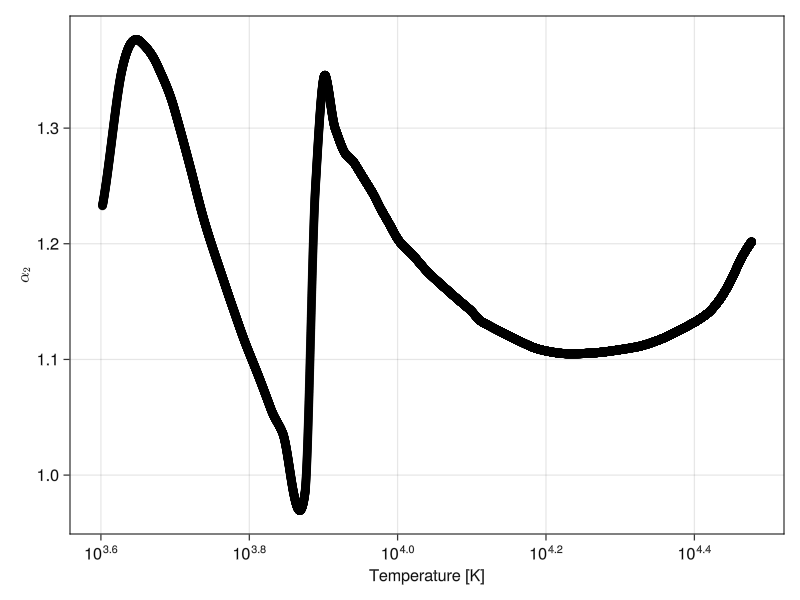
\includegraphics[scale=0.4]{plots/A_2_dependence.png}
    \caption{Dependence of the parameter $\alpha_2$ for the I band vs. the effective temperature for stars with $log g = 4$ and $[Fe/H] = -1$ dex.}
    \label{claret}
\end{figure}

\chapter{Observational data}
\section{Description of data and preprocessing}
From the OGLE \citet{udalski_optical_1992} database following two samples were analysed using aforementioned method:
\begin{itemize*}
    \item objects from the direction toward Magellanic Clouds. The sample consist of ellipsoidal stars from \citet{pawlak_ogle_2016} with objects supplemented 
    by Przemysław Mróz, 
    \item ellipsoidal variabales from the direction toward the Galactic Bulge and the Galactic Disc cross-matched by Przemysław Mróz with the Gaia DR3 
    \citep{gaia_collaboration_gaia_2022}. Sources with  {\it{rv\_amplitude\_robust}} > $100$ km/s were selected.
\end{itemize*}
The light curves used in the analysis were collected during the $4$ th season of OGLE \citet{udalski_ogle-iv_2015},
and were collected in the $I$ band.
Detailed positions of objects from the original samples in the sky are presented in the figure \ref{map}. Then for each entry the nearest Gaia source
was found and for objects with statistically significant parallax (value higher than three times it's statistical deviation) a colour-magnitude
diagram using the Gaia data was constructed and is presented in the figure \ref{HR_galactic}. Similarly a colour-magnitude diagram was constructed for
objects without statistical significant parallax, two different plots for the SMC and the LMC are presented in the figure \ref{HR_SMC}.
Most of the objects in the samples have a relatively short period ($<3$ d); a detailed period distribution
is presented in the figure \ref{periods}.
\begin{figure}
    \begin{center}
        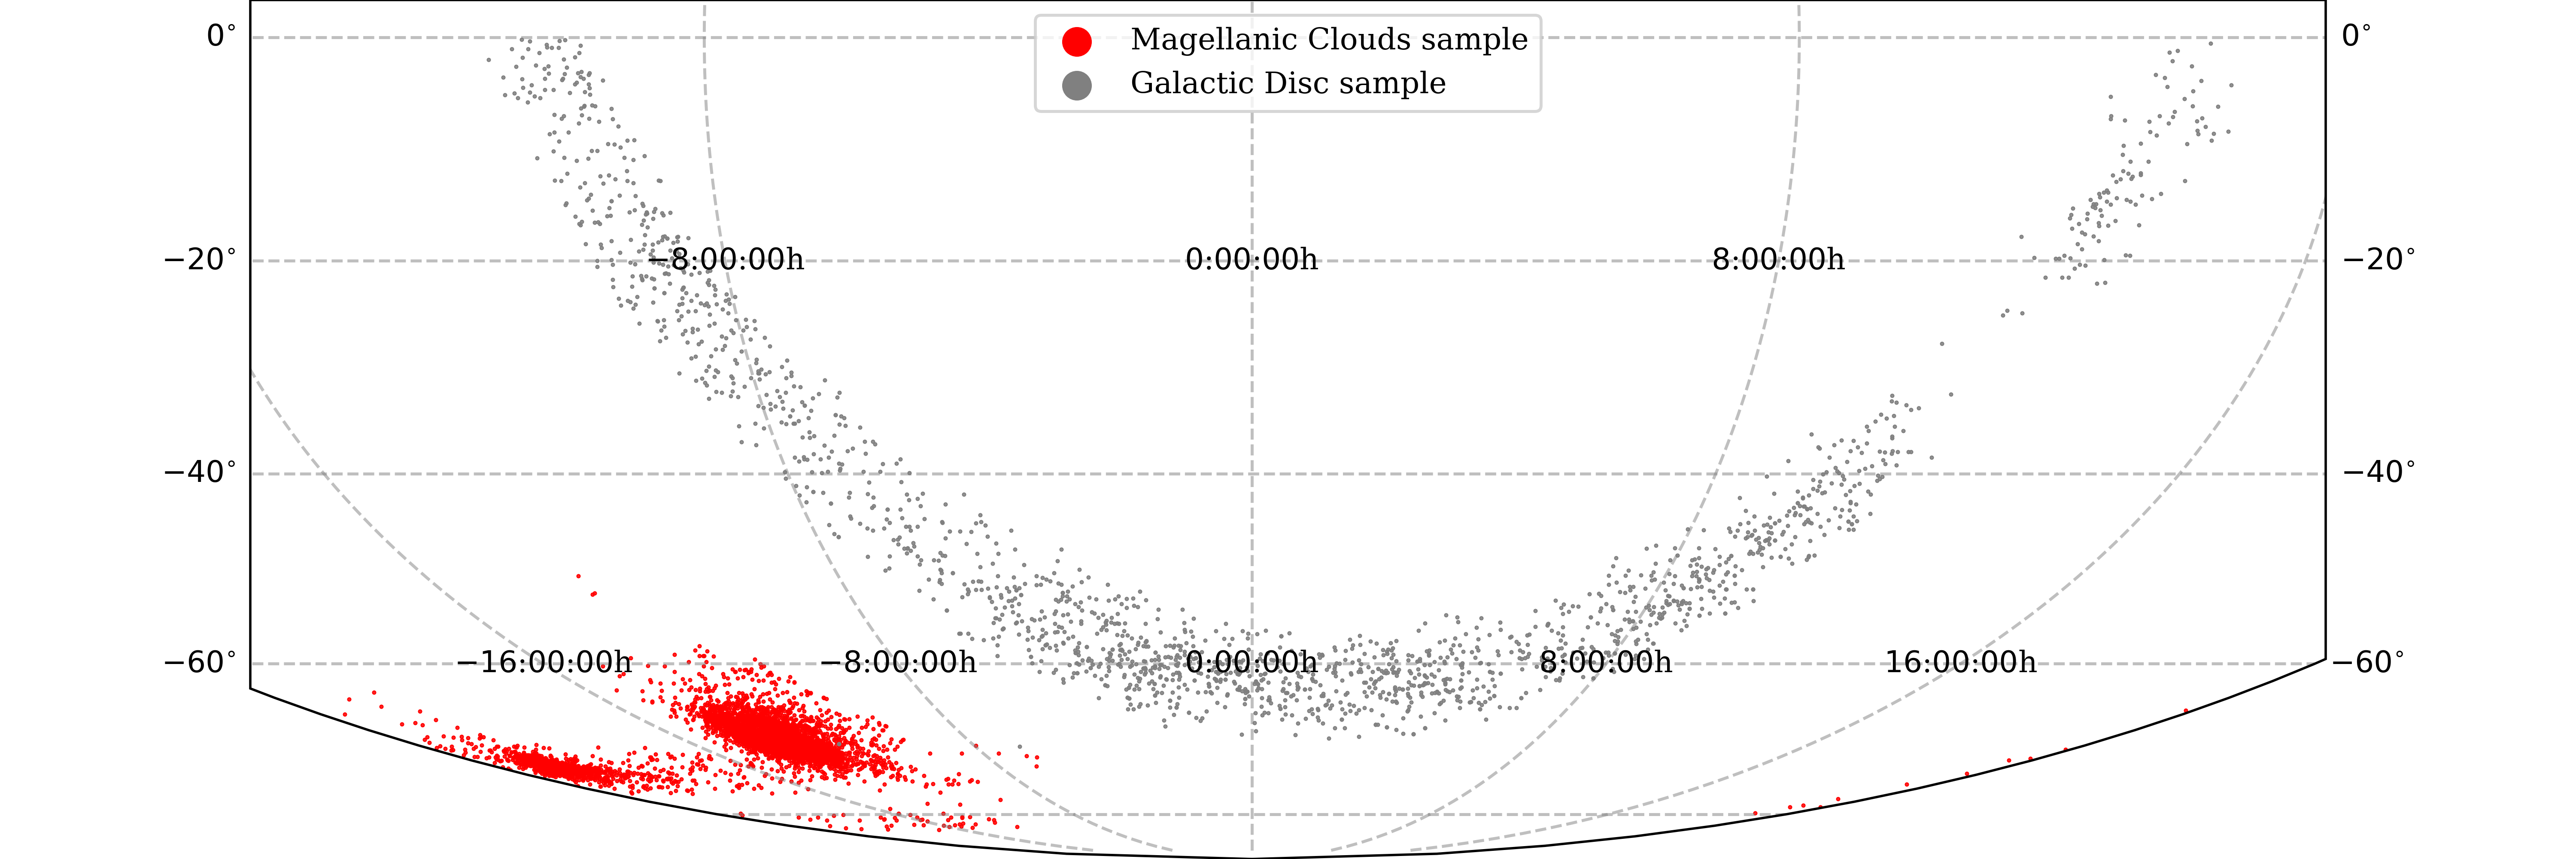
\includegraphics[scale=0.52]{plots/map_sample.png}
    \end{center}
    \caption{Positions of objects from the samples across the southern sky.}
    \label{map}
\end{figure}

\begin{figure}[H]
    \begin{center}
        \includegraphics[scale=0.6]{plots/HR_LMC_SMC.png}
    \end{center}
    \caption{A color-magnitude diagram of Gaia counterparts potentially residing in Magellanic Clouds (without statistically significant parallax).}
    \label{HR_SMC}
\end{figure}

\begin{figure}[H]
    \begin{center}
        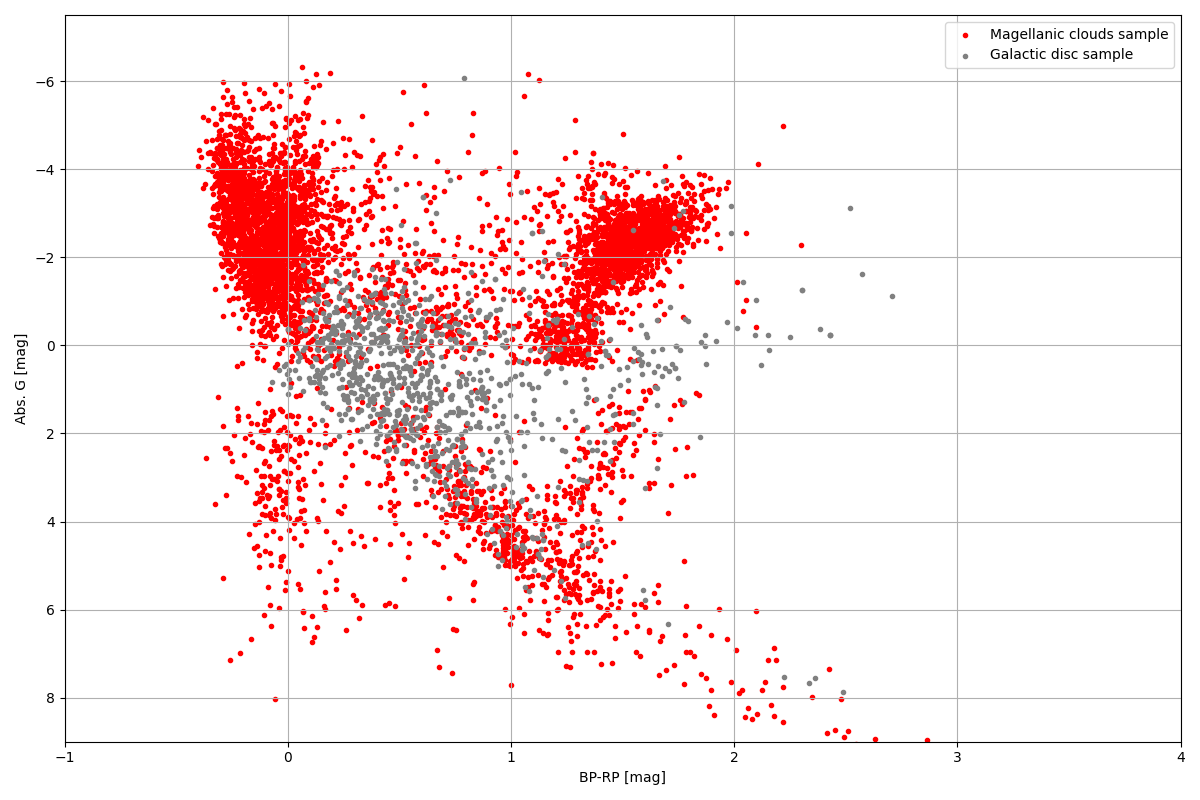
\includegraphics[scale=0.5]{plots/HR.png}
    \end{center}
    \caption{A color-magnitude diagram of Gaia counterparts with statistically significant parallax.}
    \label{HR_galactic}
\end{figure}
As a first step of preprocessing objects with brightness lower than
$17$ mag  were removed as faint stars wouldn't be suitable for a radial velocity determination with the usage of high resolution spectroscopy.
Each object was analysed using the ANOVA (analysis of variance) method \citep{schwarzenberg-czerny_advantage_1989} to determine the period.
Then each light curve was fitted with the $4$th degree harmonic model
\begin{equation}\label{harm}
    I(t)=A_0+\sum_{i=1}^4\left[ A_{1i}\sin{\left(2\pi i\frac{t}{P}\right)}+A_{2i}\cos{\left(2\pi i\frac{t}{P}\right)}\right]
\end{equation}
with the sigma clipping threshold set at $3\sigma$ allowing to determine amplitudes of coefficients from the relationship $A_i=\sqrt{A_{1i}^2+A_{2i}^2}$.
Subsequently, the minimum mass ratio $q_{mmr}$ and its lower bound $\tilde{q}_{mmr}$ were calculated and the previously described procedure of selecting candidates was carried out.
Objects with light curves indicating other type of variability then ellipsoidal one were removed together with those with period higher then
$50$ d. According to the main assumption in the analysis objects should be composed of stars nearly filling their Roche lobe, so a rather short period is suggested. The exact value of the threshold can be debated; here it is used as a mean to
remove pulsating stars that pollute the sample. After this part of the preprocessing, only $41$ objects from the first sample were left together with $22$ objects from the second sample.
\begin{figure}
    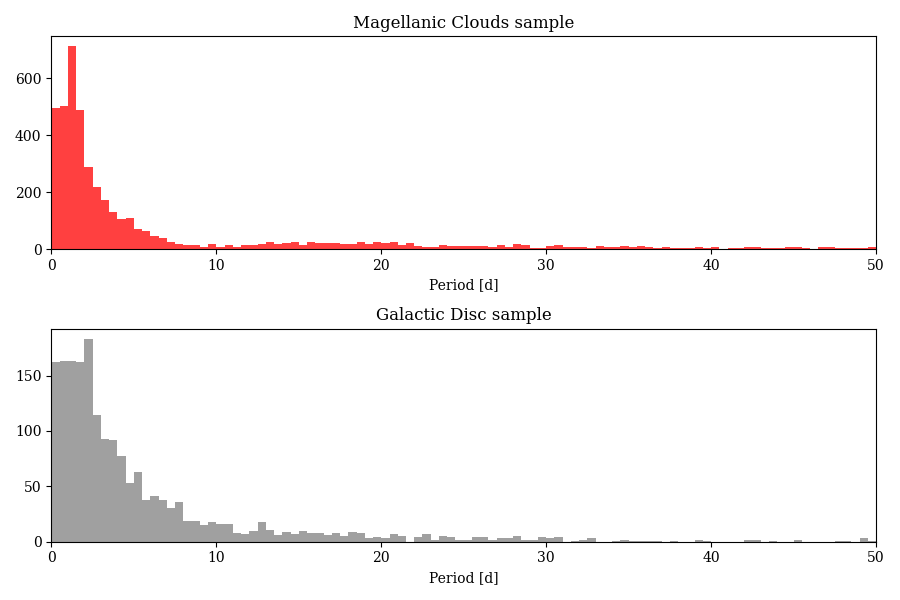
\includegraphics[scale=0.5]{plots/periods.png}
    \caption{Distribution of periods from the analysed samples.}
    \label{periods}
\end{figure}


\section{Spectral Energy Distribution}
Each object was cross-matched with the Gaia DR3 catalogue to obtain parallax (denoted $\pi_0$ together with uncertainty denoted $\sigma_{\pi}$) estimates of the objects. If the parallax was statistically significant ($\pi>3\sigma_{\pi}$)
it was used to derive the distance to the object. For objects towards Magellanic Clouds many entries lacked a statistically significant parallax, indicating that they really reside in Magellanic Clouds
and do not line up accidentally.
In this case, the distance estimate $d_0$ and the distance uncertainty $\sigma_d$ were based on \citet{jacyszyn-dobrzeniecka_ogle-ing_2016}. It is assumed that the presented distribution
of Cepheids reflects the underlying distribution of stars in the sample.
In the case of LMC and SMC the assumed distance estimates were $d_{LMC}=49.93\pm1.79$ kpc and $d_{SMC}=64.62\pm4.95$ kpc, respectively. 

To further investigate the nature of objects, a spectral energy distribution analysis was
performed with two models: a single star model and a double star model. Main goal of this type of analysis is to use a photometry from various parts of a stellar spectra to
reconstruct a whole spectral characteristic and hence infer parameters (like a temperature and a luminosity) of an object.
The single star model depends on three free parameters: a logarithm of temperature $\log_{10}T$ (expressed in kelvins), a logarithm of luminosity $\log_{10} L$ (espressed in $L_{\odot}$) and the third
parameter was either a parallax (if one was measured), or a distance if it wasn't available. In the case of the double-star model, there were two additional parameters describing the
second star $\log_{10} T_2$ and $\log_{10} L_2$. In the case of the first model star, it was assumed to be a main sequence object (MS) with $\log{g}=4$. In the double star model the primary star
was assumed to have $\log{g_1}=4$ as in the first case, while the second object was assumed to be a giant with $\log{g_2}=2$. Objects with a statistically significant parallax were assumed to have solar-like
metallicity ($Z=0.013$) as they reside inside the Galactic disc. Objects in Magellanic Clouds
were assumed to have a metallicity equal to $Z=0.010$ in the case of LMC/MBR and $Z=0.005$ in the case of SMC.
The BaSeL library of stellar spectra \citep{lejeune_standard_1998} was used to find the spectrum for any given $\log_{10}{T}$, $\log_{10} L$, $d$ 
by means of the interpolation as implemented in the Python library
\texttt{pystellibs}\footnote{https://github.com/mfouesneau/pystellibs}.
Then the theoretically calculated stellar spectrum is then processed using the \texttt{pyphot}\footnote{https://github.com/mfouesneau/pyphot} 
Python library, yielding a magnitude in a required filter.

In order to find a set of best-fitting parameters, a Bayesian approach was adopted. Let's denote a set of observed magnitudes as $\tilde{m}_i$, theoretically predicted
magnitudes as $m_i$ while errors of magnitudes as $\sigma_i$. Let's denote by $\mathcal{U}(a,b)$ a uniform distribution with the support in the form of an interval $[a,b]$ and $\mathcal{N}(\mu,\sigma^2)$ as a
normal distribution with a mean $\mu$ and a variance $\sigma^2$. In order to prepare the Bayesian model one need to specify a probability distribution that will allow to evaluate a likelihood of
data. Each of the observed magnitudes $\tilde{m}_i$ is expected to be normally distributed with a mean $m_i$ and a variance $\sigma_i^2$, while the prior distributions on each of the three parameters
are uniform in the case of $\log_{10} T$ and $\log_{10} L$, or normal in the case of a distance or a parallax. A detailed model can be written as:
\begin{equation}
    \begin{split}
    \log_{10}{T}\sim \mathcal{U}(3.31,4.6)\\
    \log_{10}{L} \sim \mathcal{U}(-3,5)\\
    d \sim \mathcal{N}(d_0,\sigma_d^2) \textrm{ or } \\
    \pi \sim \mathcal{N} (\pi,\sigma_{\pi}^2)\\
    \tilde{m}_i\sim \mathcal{N}(m_i(\log_{10} T, \log_{10} L, d ),\sigma_i^2) \textrm{ or }\\
    \tilde{m}_i\sim \mathcal{N}(m_i(\log_{10} T, \log_{10} L, \pi ),\sigma_i^2)
    \end{split}
\end{equation}
where $m_i(\log_{10} T, \log_{10} L, d )$ is written to indicate that a predicted magnitude is a function of parameters. 
Similarly, one can write down the second model together with priors for the parameters
\begin{equation}
    \begin{split}
    \log_{10}{T_1}\sim \mathcal{U}(3.31,4.6)\\
    \log_{10}{L_1} \sim \mathcal{U}(-3,5)\\
    \log_{10}{T_2}\sim \mathcal{U}(3.444,4.21)\\
    \log_{10}{L_2} \sim \mathcal{U}(-3,5)\\
    d \sim \mathcal{N}(d_0,\sigma_d^2) \textrm{ or } \\
    \pi \sim \mathcal{N} (\pi,\sigma_{\pi}^2)\\
    \tilde{m}_i\sim \mathcal{N}(m_i,\sigma_i^2)
    \end{split}
\end{equation}
where explicit dependence of $m_i$ on the parameters was hidden for clarity. In both cases, the normal distribution is truncated to positive numbers, as
negative parallax/distance solutions are not permitted. The range of a logarithm of temperature is limited due to the boundaries of the library, whereas a logarithm of luminosity is
set in the boundaries to eliminate nonphysical solutions.
Under those assumptions, a log-likelihood function can be written as 
\begin{align}
    \begin{split}
    \mathcal{L}=-\sum_i\frac{(\tilde{m}_i-m_i)^2}{2\sigma_i^2}-\frac{(d-d_0)^2}{2\sigma_d^2} \textrm{ or }\\
    \mathcal{L}=-\sum_i\frac{(\tilde{m}_i-m_i)^2}{2\sigma_i^2}-\frac{(\pi-\pi_0)^2}{2\sigma_{\pi}^2}
    \end{split}
\end{align} depending whether a distance or a parallax was used. 

Following catalogues were used to assemble SEDs:
\begin{enumerate}
\item Catalogues shared by both samples of objects:
\begin{itemize}
    \item 2MASS survey \citep{skrutskie_two_2006},
    \item Gaia DR2 \citep{gaia_collaboration_gaia_2018},
    \item VISTA Hemisphere Survey DR5 \citep{mcmahon_vizier_2021},
    \item ALLWISE/WISE survey (\citet*{wright_wide-field_2010}, \citet*{cutri_vizier_2021}),
    \item GALEX Survey \citep{bianchi_galex_2011},
    \item Denis survey  \citep{denis_vizier_2005},
    \item SkyMapper DR1/DR2 (\citet*{wolf_skymapper_2018}, \citet*{onken_skymapper_2019}),
    \item XMM Optical Monitor serendipitous sources catalog \citep{page_xmm-newton_2012}.
\end{itemize}
\item Catalogues exclusive to the Magellanic Clouds sample:
\begin{itemize}
    \item VISTA Magellanic Cloud survey DR4 \citep{cioni_vizier_2017},
    \item Spitzer SAGE survey: SMC and LMC (\citet*{meixner_spitzer_2006},\citet*{gordon_surveying_2011}),
    \item Denis catalogue of objects in Magellanic Clouds \citep{cioni_denis_2000},
    \item Magellanic Clouds Photometric Survey: SMC and LMC \citep{zaritsky_magellanic_2002,zaritsky_magellanic_2004}.
\end{itemize}
\item Catalogues exclusive to the Galactic Disc sample:
\begin{itemize}
    \item Bochum Galactic Disc survey \citep{hackstein_bochum_2015},
    \item AAVSO Photometric All Sky Survey DR9 \citep{henden_apass_2015},
    \item VISTA Variables in Via Lactea Survey DR2 \citep{minniti_vizier_2017},
    \item GLIMPSE source catalog \citep{spitzer_science_vizier_2009}.
\end{itemize} 
\end{enumerate}
In the case of Magellanic Clouds, extinction estimates were based on the map \citep{skowron_ogle-ing_2021}, while in the case of Galactic disc extinction it
was obtained using the \texttt{ mwdust} \citep{bovy_galactic_2016} Python library with the 3D dust map being a combination of \citep{green_3d_2019}, \citep{greiner_unusually_2001},
\citep{drimmel_three-dimensional_2003}.
As the OGLE does not cover positions of all objectts, those without an estimated extinction were assumed to be zero.
In the calculations, the Cardelli extinction law \citep{cardelli_relationship_1989} with $R_V=3.1$ was assumed
and the Python implementation from \texttt{extinction}\footnote{https://extinction.readthedocs.io/en/latest/index.html} was used.
Using the described setup, the MCMC Python-based library \texttt{emcee}\footnote{https://emcee.readthedocs.io/en/stable/} \citep{foreman-mackey_emcee_2013}
was used to construct the set\footnote{https://github.com/Wesenheit/Iris} of routines used to sample from the posterior of the models, providing estimates of parameters together
with associated uncertainties.
Other packages used in the study are \texttt{astroquery} \citep{ginsburg_astroquery_2019},
\texttt{corner} \citep{foreman-mackey_cornerpy_2016} and \texttt{astropy} \citep{astropy_collaboration_astropy_2022}.
Each sampling was carried out with $32$ walkers for $2000$ steps (with $750$ burn in); in the case of a double model, each sampling 
was followed by a second one with starting conditions sampled from the first chain. 
A chain convergence was checked with a corner plot, two example plots are presented in the figure
\ref{corner_1}.
In order to help to decide between models
the BIC score was used 
\begin{equation}
    BIC=k\log{n}-2\mathcal{L}
\end{equation} where $k$ is a number of estimated parameters and $n$ is a number of data points. From all objects thirteen were selected based on the high quality fit with the single star model.
One of the objects was selected due to the observed X-ray emission 
that can indicate existence of the accretion disc. The key parameters of the objects are listed in the table \ref{objects}.
\begin{table}[H]
    \scriptsize
    \centerline{
    %\resizebox{\columnwidth}{!}{
    \begin{tabular}{llllllllllll}
    \hline
    Name&     Period [d]&     $q_{mmr}$ & $\tilde{q}_{mmr}$   &    RA [deg]        &  DEC [deg]        &   $A_0$    &      $A_1$ &   $A_2$     &    $A_3$     &     $A_4$  & $\pi_0$ [mas] \\
    \hline
    \hline
    BLG986.08.7     & $0.5132$  & $1.46$ & $1.03$  & $260.451241$ & $-43.019464$ & $12.192$ & $0.0028$  & $0.0985$ & $0.0039$  & $0.0093$ & $1.20$ \\[0.1cm]
    GD2246.03.18414 & $0.4270$ & $2.29$ & $1.55$ & $179.327372$ & $-57.091968$ & $12.0764$ & $0.0045$  & $0.1090$ & $0.0030$ & $0.0106$  & $1.41$ \\[0.1cm]
    GD1097.20.23000 & $0.4570$ & $9.73$ & $5.18$  & $252.108419$ & $-44.137004$ & $11.782$ & $0.0008$ & $0.1414$  & $0.0029$ & $0.0200$  &  $1.78$ \\[0.1cm]
    GD1448.27.17    & $1.2410$  & $1.77$ & $1.23$ & $139.969949$ & $-45.759178$ & $11.875$ & $0.0115$  & $0.1035$ & $0.0030$  & $0.0056$  &  $0.77$ \\[0.1cm]
    BLG931.27.36745 & $0.7050$   & $2.44$  & $1.63$ & $261.74489$  & $-40.31792$  & $11.633$ & $0.0033$ & $0.1113$ & $0.0026$ & $0.0105$ & $1.46$     \\[0.1cm]
    GD1070.18.22288 & $45.1467$  & $7.41$ & $3.73$ & $257.007546$ & $-41.048747$ & $11.369$ & $0.0091$  & $0.1362$  & $0.0043$  & $0.0049$ &   $1.03$ \\[0.1cm]
    LMC574.11.3407  & $0.2551$ & $1.48$ & $1.03$ & $80.1415$    & $-63.185667$ & $16.919$ & $0.0064$ & $0.0989$ & $0.0013$ & $0.0092$  &  $0.45$ \\[0.1cm]
    LMC606.30.48    & $0.2698$   & $1.67$  & $1.11$ & $92.27575$   & $-63.376167$ & $15.906$ & $0.0141$  & $0.1019$ & $0.0038$  & $0.0122$ &   $0.52$ \\[0.1cm]
    LMC751.15.2886  & $0.3753$ & $1.70$ & $1.16$  & $98.082958$  & $-66.307861$ & $16.958$    & $0.0090$  & $0.1024$ & $0.0012$ & $0.0121$  &  $0.18$ \\[0.1cm]
    MBR108.18.3     & $0.2947$  & $1.49$ & $1.02$ & $33.257292$  & $-72.993167$ & $13.376$ & $0.0063$ & $0.0989$ & $0.0033$  & $0.0128$  &  $1.10$ \\[0.1cm]
    MBR236.09.433   & $0.4398$  & $1.51$ & $1.07$ & $50.642958$  & $-80.540667$ & $14.585$ & $0.0024$ & $0.0994$  & $0.0028$ & $0.0089$  &  $0.47$ \\[0.1cm]
    SMC711.22.1068  & $0.4466$  & $2.35$  & $1.56$ & $9.833875$   & $-70.378028$ & $13.226$ & $0.0029$  & $0.1104$ & $0.0053$  & $0.0154$ & $0.66$     \\[0.1cm]
    SMC720.28.40576 & $0.5674$ & $4.29$  & $2.56$ & $11.938042$  & $-73.13625$  & $16.367$  & $0.0017$ & $0.1246$ & $0.0037$  & $0.0035$ &  $-$    \\[0.1cm]
    SMC742.26.330   & $0.3453$ & $1.68$ & $1.12$ & $350.85925$  & $-77.530417$ & $13.864$ & $0.0042$   & $0.1020$ & $0.0049$ & $0.0074$ & $1.07$   \\[0.1cm]
    \hline
    \end{tabular}
    %}
    }
    \caption{Selected objects together with period, estimated mass ratios, coordinates, Fourier coefficients ($A_i$) and parallax from Gaia DR3.}\label{objects}
\end{table}
What should be emphasised here is the meaning of the BIC score. Little is assumed about objects; especially, the best fitting
$\log{g}$/Z is not investigated, which can be crucial to obtain a high quality spectral fit. Due to this effect, it is unreasonable to calculate the values of $\chi^2$ and compare them
between objects, as few of them can be better fitted with the given metallicity/$\log{g}$
(for example ultraviolet observations can be sensitive not only to the temperature of the star but also to its metallicity).
Even if some objects won't be accuratly described, it is still possible to reliable assess if there are one or more stars contributing to the spectra.
The SED fits of the single model together with light curves are presented in the Appendix A. Each subsection consists of the phased light curve, the
SED fit plot, the corner plot for the posterior distribution and other relevant data.
\newpage
\begin{figure}
    \begin{subfigure}{1\textwidth}
        \centering
       \includegraphics[scale=0.4]{plots/GD1070.18.22288_double_corner_emcee.png}
       \label{fig:Ng1} 
    \end{subfigure}
    
    \begin{subfigure}{1\textwidth}
        \centering
       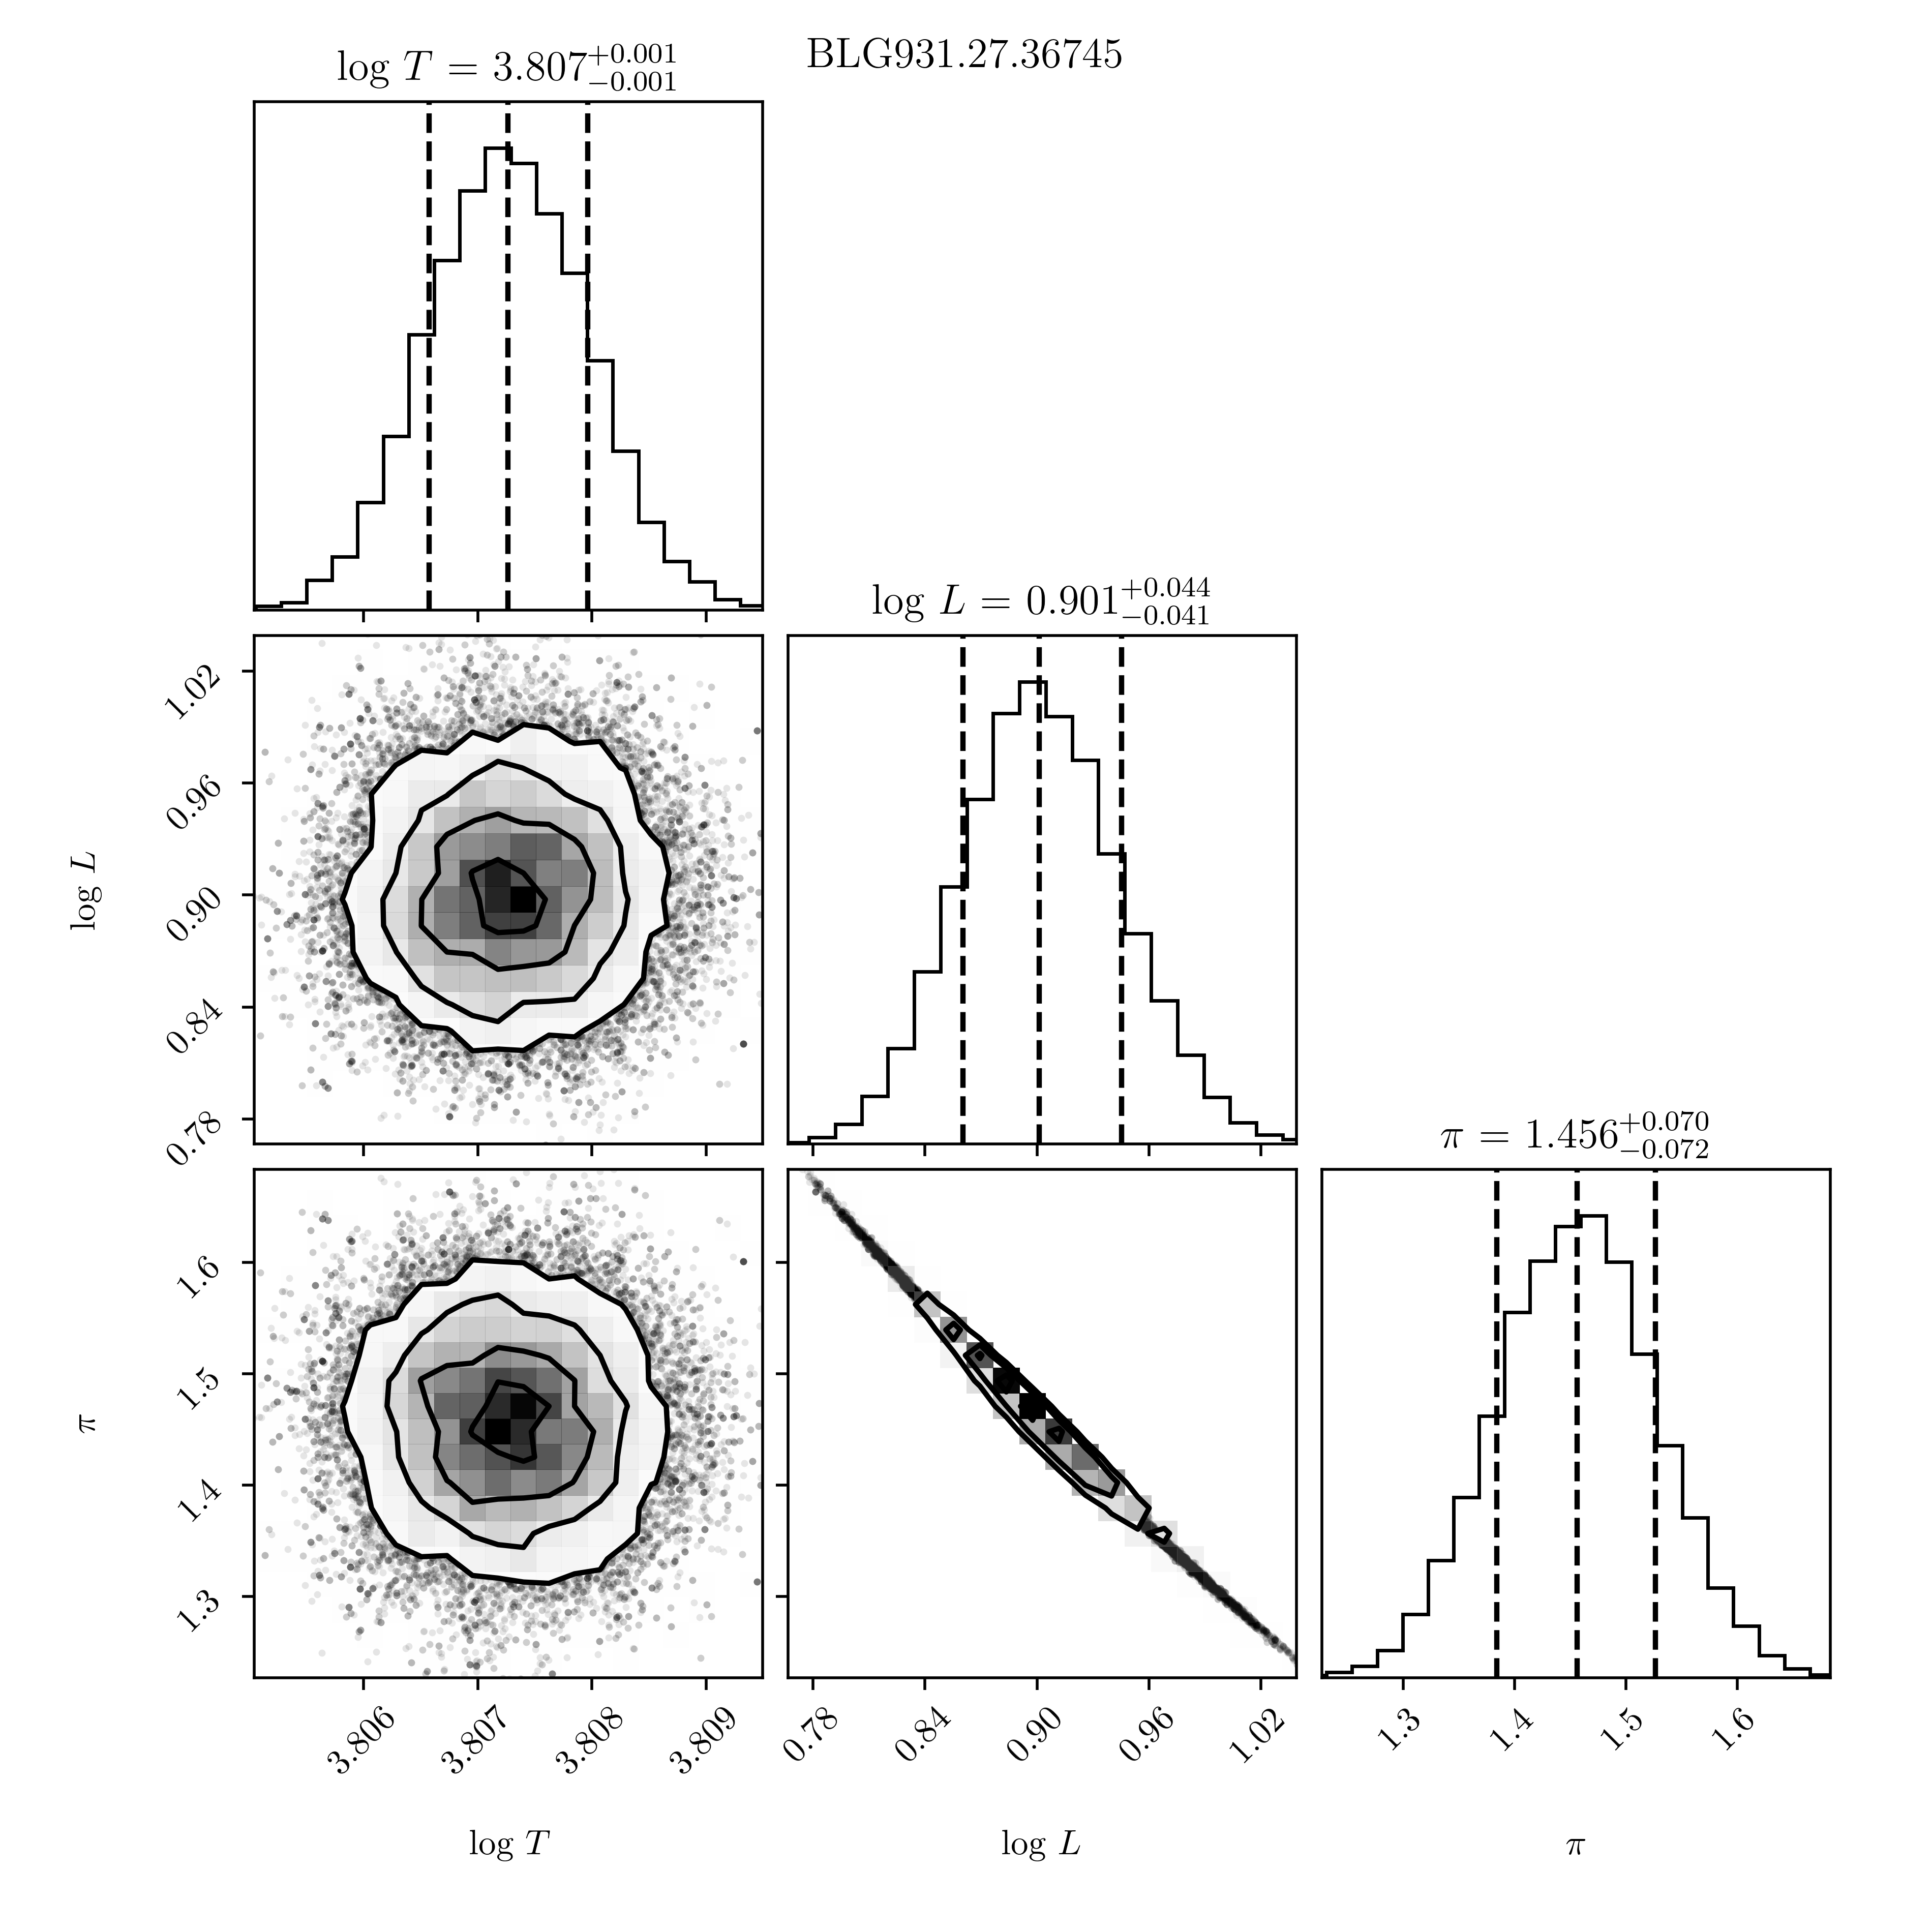
\includegraphics[scale=0.5]{plots/BLG931.27.36745_simple_corner_emcee.png}
    \end{subfigure}
    \caption{Posterior distribution from MCMC simulations for GD1070.18.22288 (double star model)
    and BLG931.27.36745 (single star model).}\label{corner_1}
\end{figure}
    %
\chapter{Results}
\section{Physical parameters of objects}
Each of the fourteen final objects was further investigated using available data to determine the physical properties.
Of all objects, twelve are spectral type G or F, one object is spectral type O, while the last is composed of two stars.
Thirteen stars from the list have a measured parallax from the Gaia DR3 while one of the objects is located in the SMC.
%Eleven objects were selected on the basis of a good fit with the single star model, while one was selected because of counterpart emission in X-ray.

For each entry, the mass of the object was estimated using the PARSEC
\citep{bressan_span_2012} evolutionary tracks. Assuming solar-like metallicity,
simple approximate fits were obtained by choosing a best-fitting entry from the PARSEC track using temperature and luminosity estimates from SED fits.
Each model was fitted with a track using the nearest metallicity from PARSEC data ($Z=0.014$ in the case of a objects inside the Galactic Disc and $Z=0.004$ in the case of the SMC).
As it was assumed that each object should be a
MS star, parts of evolutionary tracks before the beginning of the ZAMS were discarded.
\begin{table}[H]
    \footnotesize
    \centerline{
    \centering
    \begin{tabular}{lllllll}
    \hline
    Name& $T$ [K] & $\log_{10} L/L_{\odot}$ &$E(B-V)$ & $d$ [kpc] & BIC & $M_{PARSEC}$ [$\textrm{M}_\odot$]\\
    \hline
    \hline
    BLG986.08.7     & $6190^{+26}_{-25}$ & $0.825^{+0.011}_{-0.012}$ & $0.226$ & $0.83\pm 0.01$ & $729.8$ & $1.4$ \\[0.1cm]
    GD2246.03.18414 & $6974^{+21}_{-28}$ & $0.806 \pm 0.008$ & $0.273$ & $0.71\pm 0.01$ & $586.3$ & $1.45$ \\[0.1cm]
    GD1097.20.23000 & $6126\pm 13$ & $0.626^{+0.007}_{-0.006}$ & $0.221$  & $0.56\pm 0.008$ & $197.8$ & $1.2$ \\[0.1cm]
    GD1448.27.17    & $8516^{+59}_{-64}$ & $1.863\pm 0.013$ & $0.611$  & $1.30\pm 0.02$ & $215.8$ & $2.3$ \\[0.1cm]
    BLG931.27.36745 & $6416\pm 10$ & $0.901^{+0.044}_{-0.041}$ & $0.199$  & $0.69^{+0.04}_{-0.03}$ & $206.1$ & $1.4$ \\[0.1cm]
    LMC574.11.3407  & $4740\pm 24$ & $-0.349^{+0.153}_{-0.124}$ & $0.034$  & $2.21^{+0.42}_{-0.29}$ & $849.3$ & $-$ \\[0.1cm]
    LMC606.30.48    & $5516\pm 25$ & $-0.053\pm 0.066$ & $0.047$  & $1.93^{+0.15}_{-0.13}$ & $184$ & $0.85$ \\[0.1cm]
    LMC751.15.2886  & $6068\pm 23$ & $0.392^{+0.342}_{-0.241}$ & $-$  & $5.39^{+2.60}_{-1.31}$ & $470.3$ & $1.1$ \\[0.1cm]
    MBR108.18.3     & $5884\pm 6$ & $0.228\pm 0.011$ & $-$  & $0.91\pm 0.01$ & $3333.3$ & $1.0$ \\[0.1cm]
    MBR236.09.433   & $6471\pm 10$ & $0.717\pm 0.027$ & $-$  & $2.12\pm 0.07$ & $592.1$ & $1.35$ \\[0.1cm]
    SMC711.22.1068  & $6771\pm 5$ & $0.852^{+0.017}_{-0.015}$ & $0.021$  & $1.52\pm 0.03$ & $707.4$ & $1.45$ \\[0.1cm]
    SMC720.28.40576 & $34079^{+536}_{-496}$ & $4.366^{+0.069}_{-0.071}$ & $0.095$  & $-$ & $168.8$ & $16$ \\[0.1cm]
    SMC742.26.330   & $5808\pm 6$ & $0.356\pm 0.010$ & $-$  & $0.93\pm0.01$ & $2539.4$ & $1$ \\[0.1cm]
    \hline
    \end{tabular}
    }
    \caption{Estimated physical parameters of objects using the single star model together with PARSEC mass estimates and extinction estimates.}\label{objects_fit}
\end{table}

\section{Radial velocity semi-amplitude estimation from Gaia DR3 data}
Half of the objects in the final list have available high-quality radial velocity information that is normally computed for bright stars from the Gaia DR3 catalogue.
While the estimate of the radial velocity is based on the median of measurements, 
the error of this estimate is based on the epoch standard deviation. According to \citet{katz_gaia_2022} the radial velocity error $\delta v$ 
is calculated via the equation
\begin{align}
    \delta v=\sqrt{\sigma_{med}^2+0.11^2}\\
    \sigma_{med}=\sqrt{\frac{\pi}{2}}\frac{\sigma}{\sqrt{N}}
\end{align}
where $\sigma$ is a standard deviation of the radial velocity and $N$ stands for a number of transits used to compute radial velocity. This simple formula allows to obtain variance of 
radial velocity measurements as 
\begin{equation}
    \sigma^2=\frac{2N}{\pi}\left((\delta v)^2-0.11^2\right).
\end{equation}
It can be proven (for details see Appendix B) that if one assumes error is dominated by a sinusoidal radial movement with a semi-amplitude $K$,
a variance of velocity will be equal to
\begin{equation}
    \sigma^2=\frac{K^2}{2}.
\end{equation}
This observation can be used to estimate a semi-amplitude of velocity using Gaia measurements (denoted from here as $K_{\textrm{Gaia}}$) as 
\begin{equation}
    K_{Gaia}=\sqrt{\sigma^2}\sqrt{2}=2\sqrt{\frac{N}{\pi}\left((\delta v)^2-0.11^2\right)}
\end{equation}
This radial velocity amplitude is used then to calculate a binary mass function using the definition 
\begin{equation}\label{mass}
    f(M_1,M_2,i)=\frac{M_2^3 \sin{i}^3}{(M_1+M_2)^2}=\frac{K^3 P}{2\pi G}
\end{equation}
where $P$ denotes a orbital period while $G$ is the gravitational constant. For each object with a radial velocity estimation, a mass function was obtained
and presented in the table \ref{mass_function_table} with other relevant parameters.
For each object with a PARSEC mass estimate, a lower boundary of a companion mass was calculated by solving the equation \ref{mass}
with $\sin{(i)}=1$ and placed in the table as $M_{min}$.

In \citet{katz_gaia_2022} a criterion was presented that allows to test whether an object is variable in radial velocity, based on values of {\it{rv\_chisq\_pvalue}}
and {\it{rv\_renormalised\_gof}}. The criterion states that objects with $N>10$, $T_{eff}\in [3900,8000]$ K,{\it{rv\_chisq\_pvalue}}$<0.01$ and {\it{rv\_renormalised\_gof}}$>4$
can be safely considered to be variable in radial velocity. Each candidate was tested using described method,
and only two entries (BLG931.27.36745 and GD1097.20.23000) cannot be safely assumed to be variable in the radial velocity as they were not observed
enough times. This observation is the first good sign that selected candidates really are binary in nature and the sample is not polluted, i.e. by pulsating stars.
\begin{table}[H]
    \footnotesize
    \centering
    %\def\arraystretch{1.5}
    \setlength{\tabcolsep}{3pt}
    \begin{center}
    \centerline{
    \begin{tabular}{llllllll}
    \hline
    Name & Period [d]& $RV$ [km/s]&$N$ & $\delta v$  [km/s]   & $K_{Gaia}$ [km/s]  & $f(M_1,M_2,i)$ [M$_{\odot}$]& $M_{min}$ [M$_{\odot}$]\\
%    GD1549.19.348   & $2.8224$   & $36.72$ & $21$ & $8.64$  & $44.67$   & $0.026$ &\\
    \hline
    \hline
    GD2246.03.18414 & $0.4270$ & $27.68$ & $25$ & $23.03$ & $129.93$ & $0.097$  & $0.79$ \\[0.1cm]
    GD1097.20.23000 & $0.4570$ & $36.5$  & $10$ & $21.03$ & $75.03$  & $0.020$  & $0.37$\\[0.1cm]
    BLG986.08.7     & $0.5132$  & $-1.69$ & $15$ & $18.11$ & $79.14$   & $0.026$  & $0.43$\\[0.1cm]
    BLG931.27.36745 & $0.7050$   & $-4.35$ & $8$  & $14.81$ & $47.26$  & $0.0077$ & $0.28$\\[0.1cm]
    GD1448.27.17    & $1.2410$  & $33.08$ & $22$ & $7.69$  & $40.69$  & $0.0086$ & $0.40$\\[0.1cm]
    GD1070.18.22288 & $45.1467$  & $38.71$ & $20$ & $7.66$  & $38.65$  & $0.27$  & -- \\[0.1cm]
    \hline
    \end{tabular}
    }
    \end{center}
    
    \caption{Estimated mass functions together with other relevant parameters.}\label{mass_function_table}
\end{table}
%\begin{figure}[H]
%    \begin{center}
%        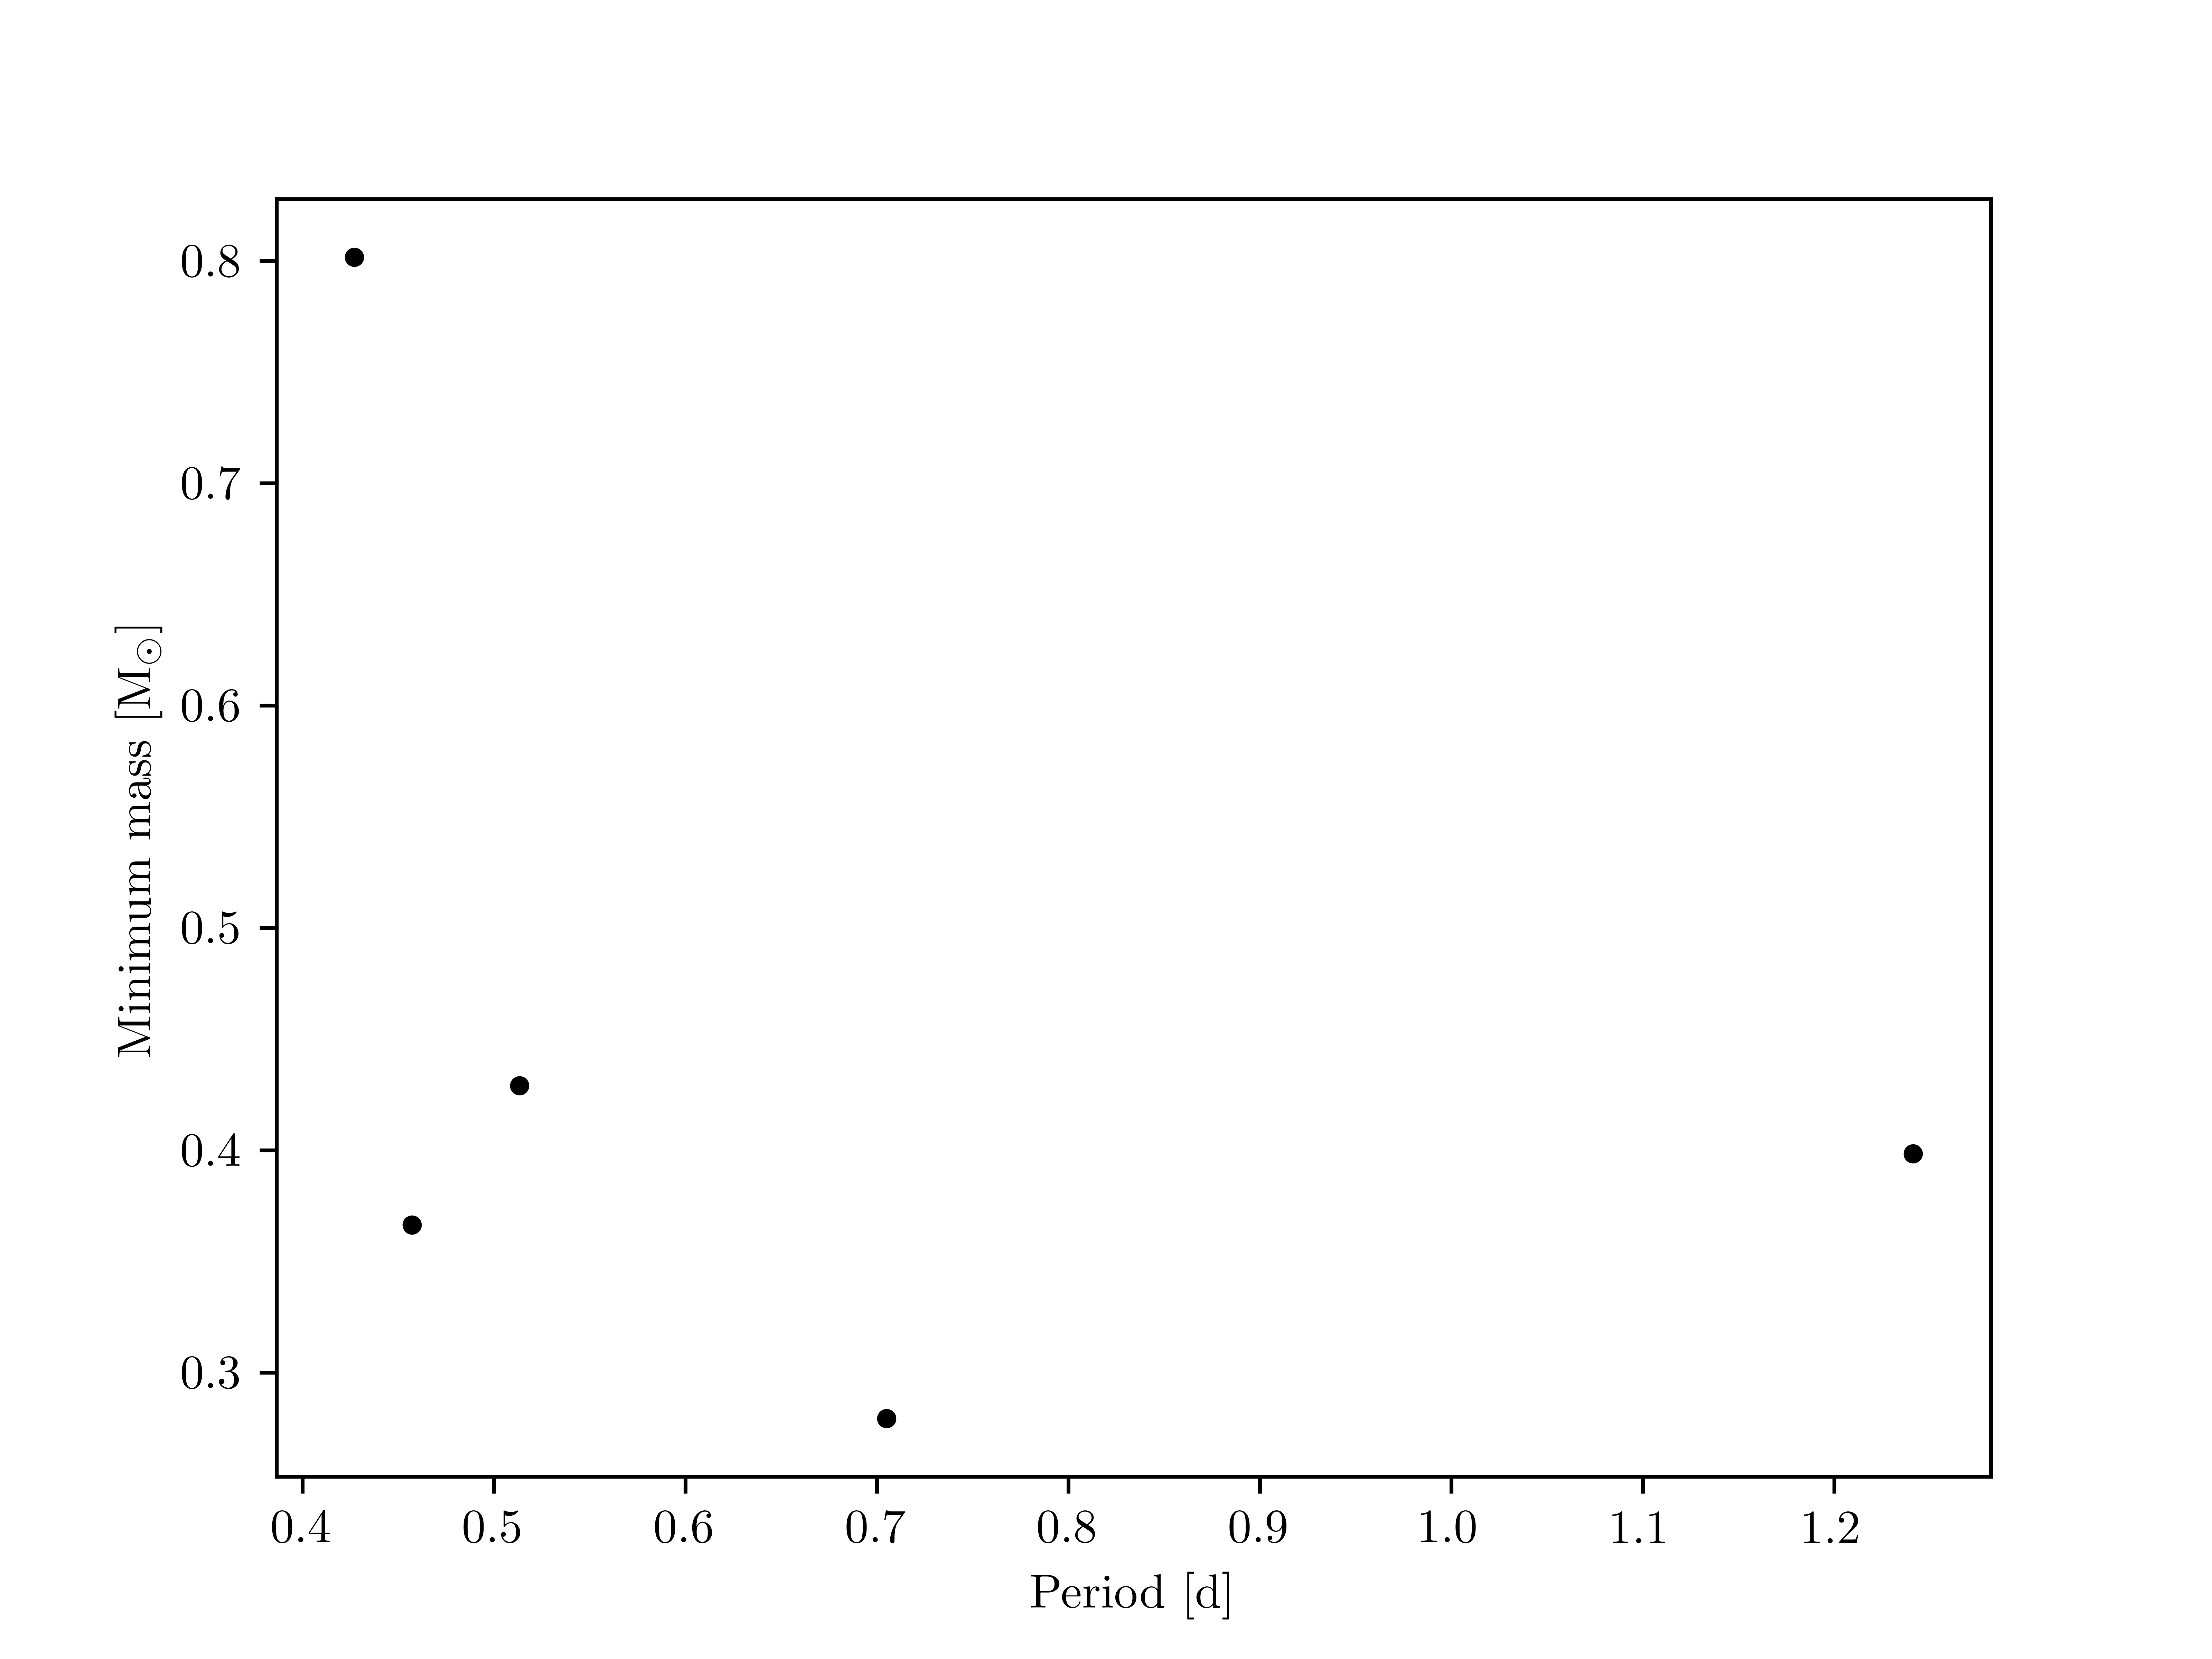
\includegraphics{plots/mass_minimum_estimate.png}
%    \end{center}
%    \caption{Lower bound of companions mass.}\label{lower_mass}
%\end{figure}

\section{Detailed analysis of objects}
In this section, a detailed characteristic of individual objects will be provided. It will be divided into $3$ subsections, where the first two will quickly cover the information
available for objects GD1070.18.22288 and SMC720.28.40576 while the third will be dedicated to the rest.
\subsection{GD1070.18.22288}
\begin{figure}[H]
    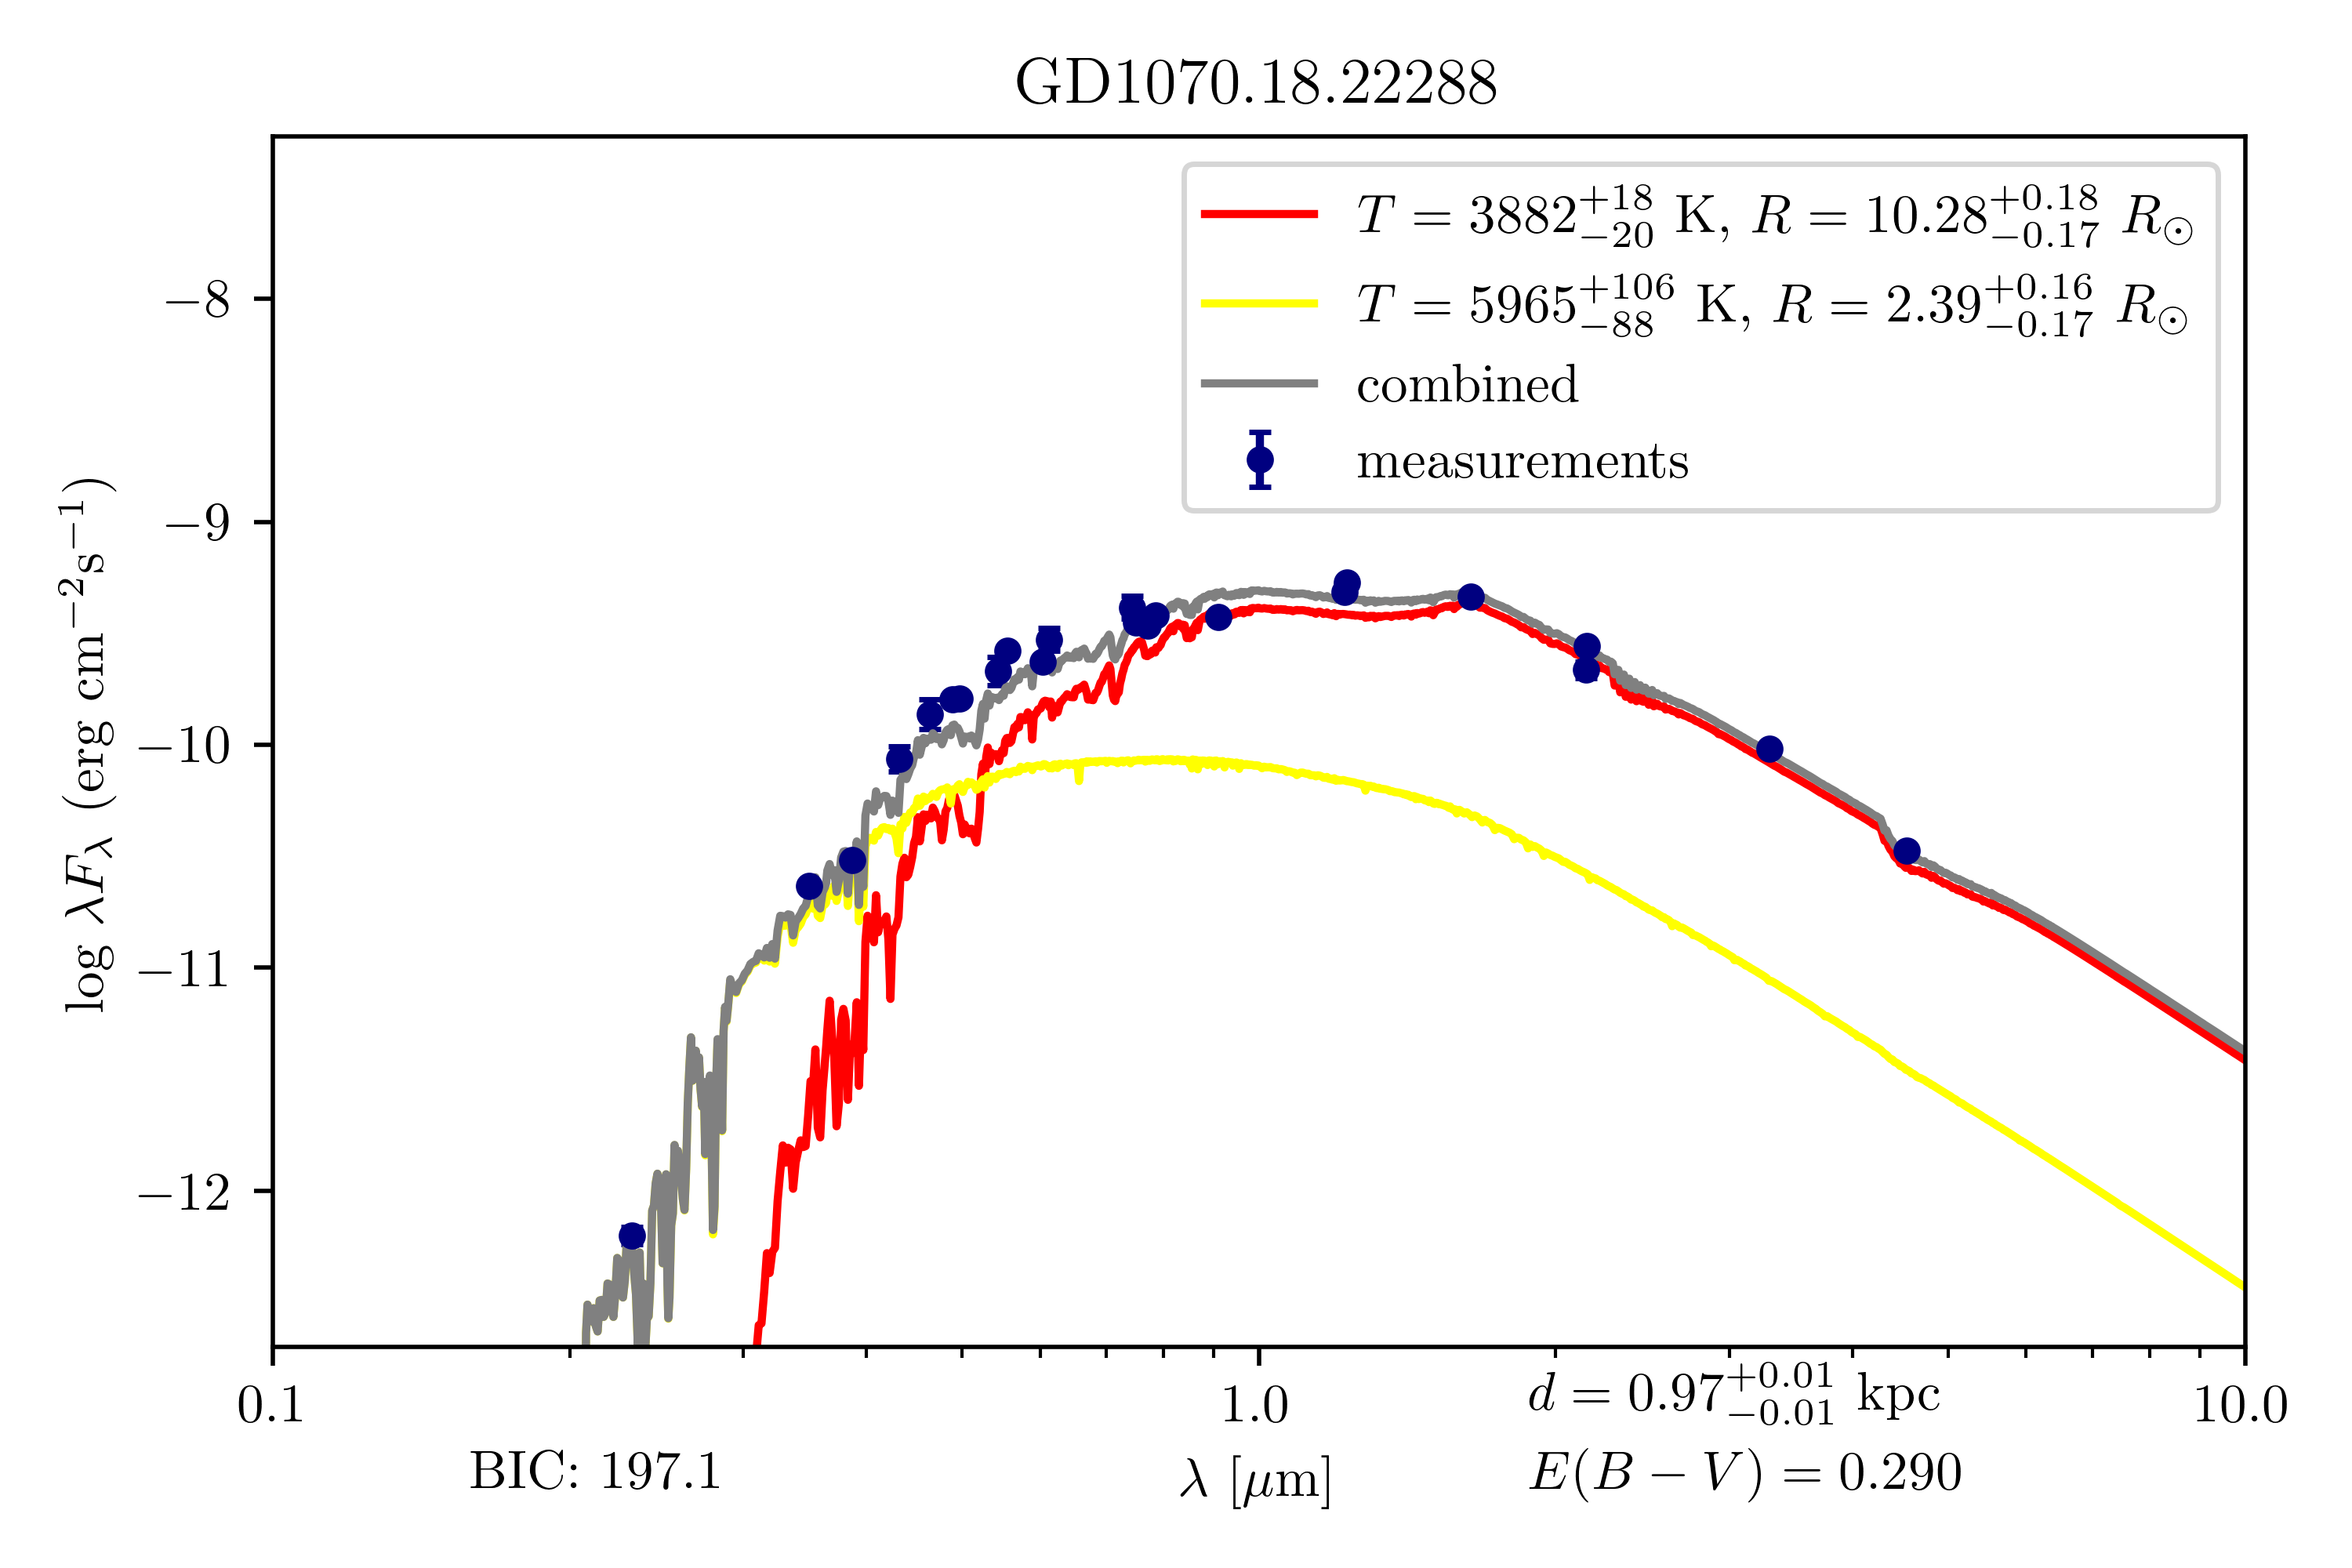
\includegraphics{plots/GD1070.18.22288/GD1070.18.22288_double_emcee.png}
    \caption{Spectral Energy Distribution fit for GD1070.18.22288 using a model with two components.}\label{GD1070SED}
\end{figure}
GD1070.18.22280 has the longest period compared to other selected objects with $P\approx 45$ d and was listed as a plausible candidate only because of the reported X-ray emission.
Due to an excess amount of observations in many parts of the spectra it was possible to obtain a high-quality spectral energy distribution fit that revealed two sources with different temperatures;
detailed distribution can be seen in the figure \ref{GD1070SED}.
One of the objects with a rather low temperature of
$T\approx 3800$ K has the radius $R\approx 10$ $\textrm{R}_{\odot}$ and was quite far from any evolutionary track in the PARSEC database. This can indicate
that was stripped in the past by it's companion.
The position of the cold companions in the HR diagram is presented in the figure \ref{HR_cold}.
The object can also be found in the ASAS-SN database \citep{jayasinghe_asas-sn_2019} under the identification number J170801.81-410255.6 where it is classified
as a rotational variable star with half of the period found in this work. The ASAS-SN observed it in the $V$ and SDSS $g$ bands, allowing light curves to be compared with the OGLE one.
Furthermore, the object was observed in the SDSS $i$ band by the Bochum disc survey \citep{hackstein_bochum_2015}. The comparison between all light curves can be found in the graph \ref{comp}.
ASAS-SN observations in the $g$ band can be traced back to $2016$ and allow one to get better insight into the nature of the object.
The evolution of the light curve over time is presented in the graph \ref{evolution}.
%The object also has the highest value of the mass function of the whole sample that is equal to $\sim 0.25 \textrm{M}_{\odot}$. 

\begin{figure}%[t]
    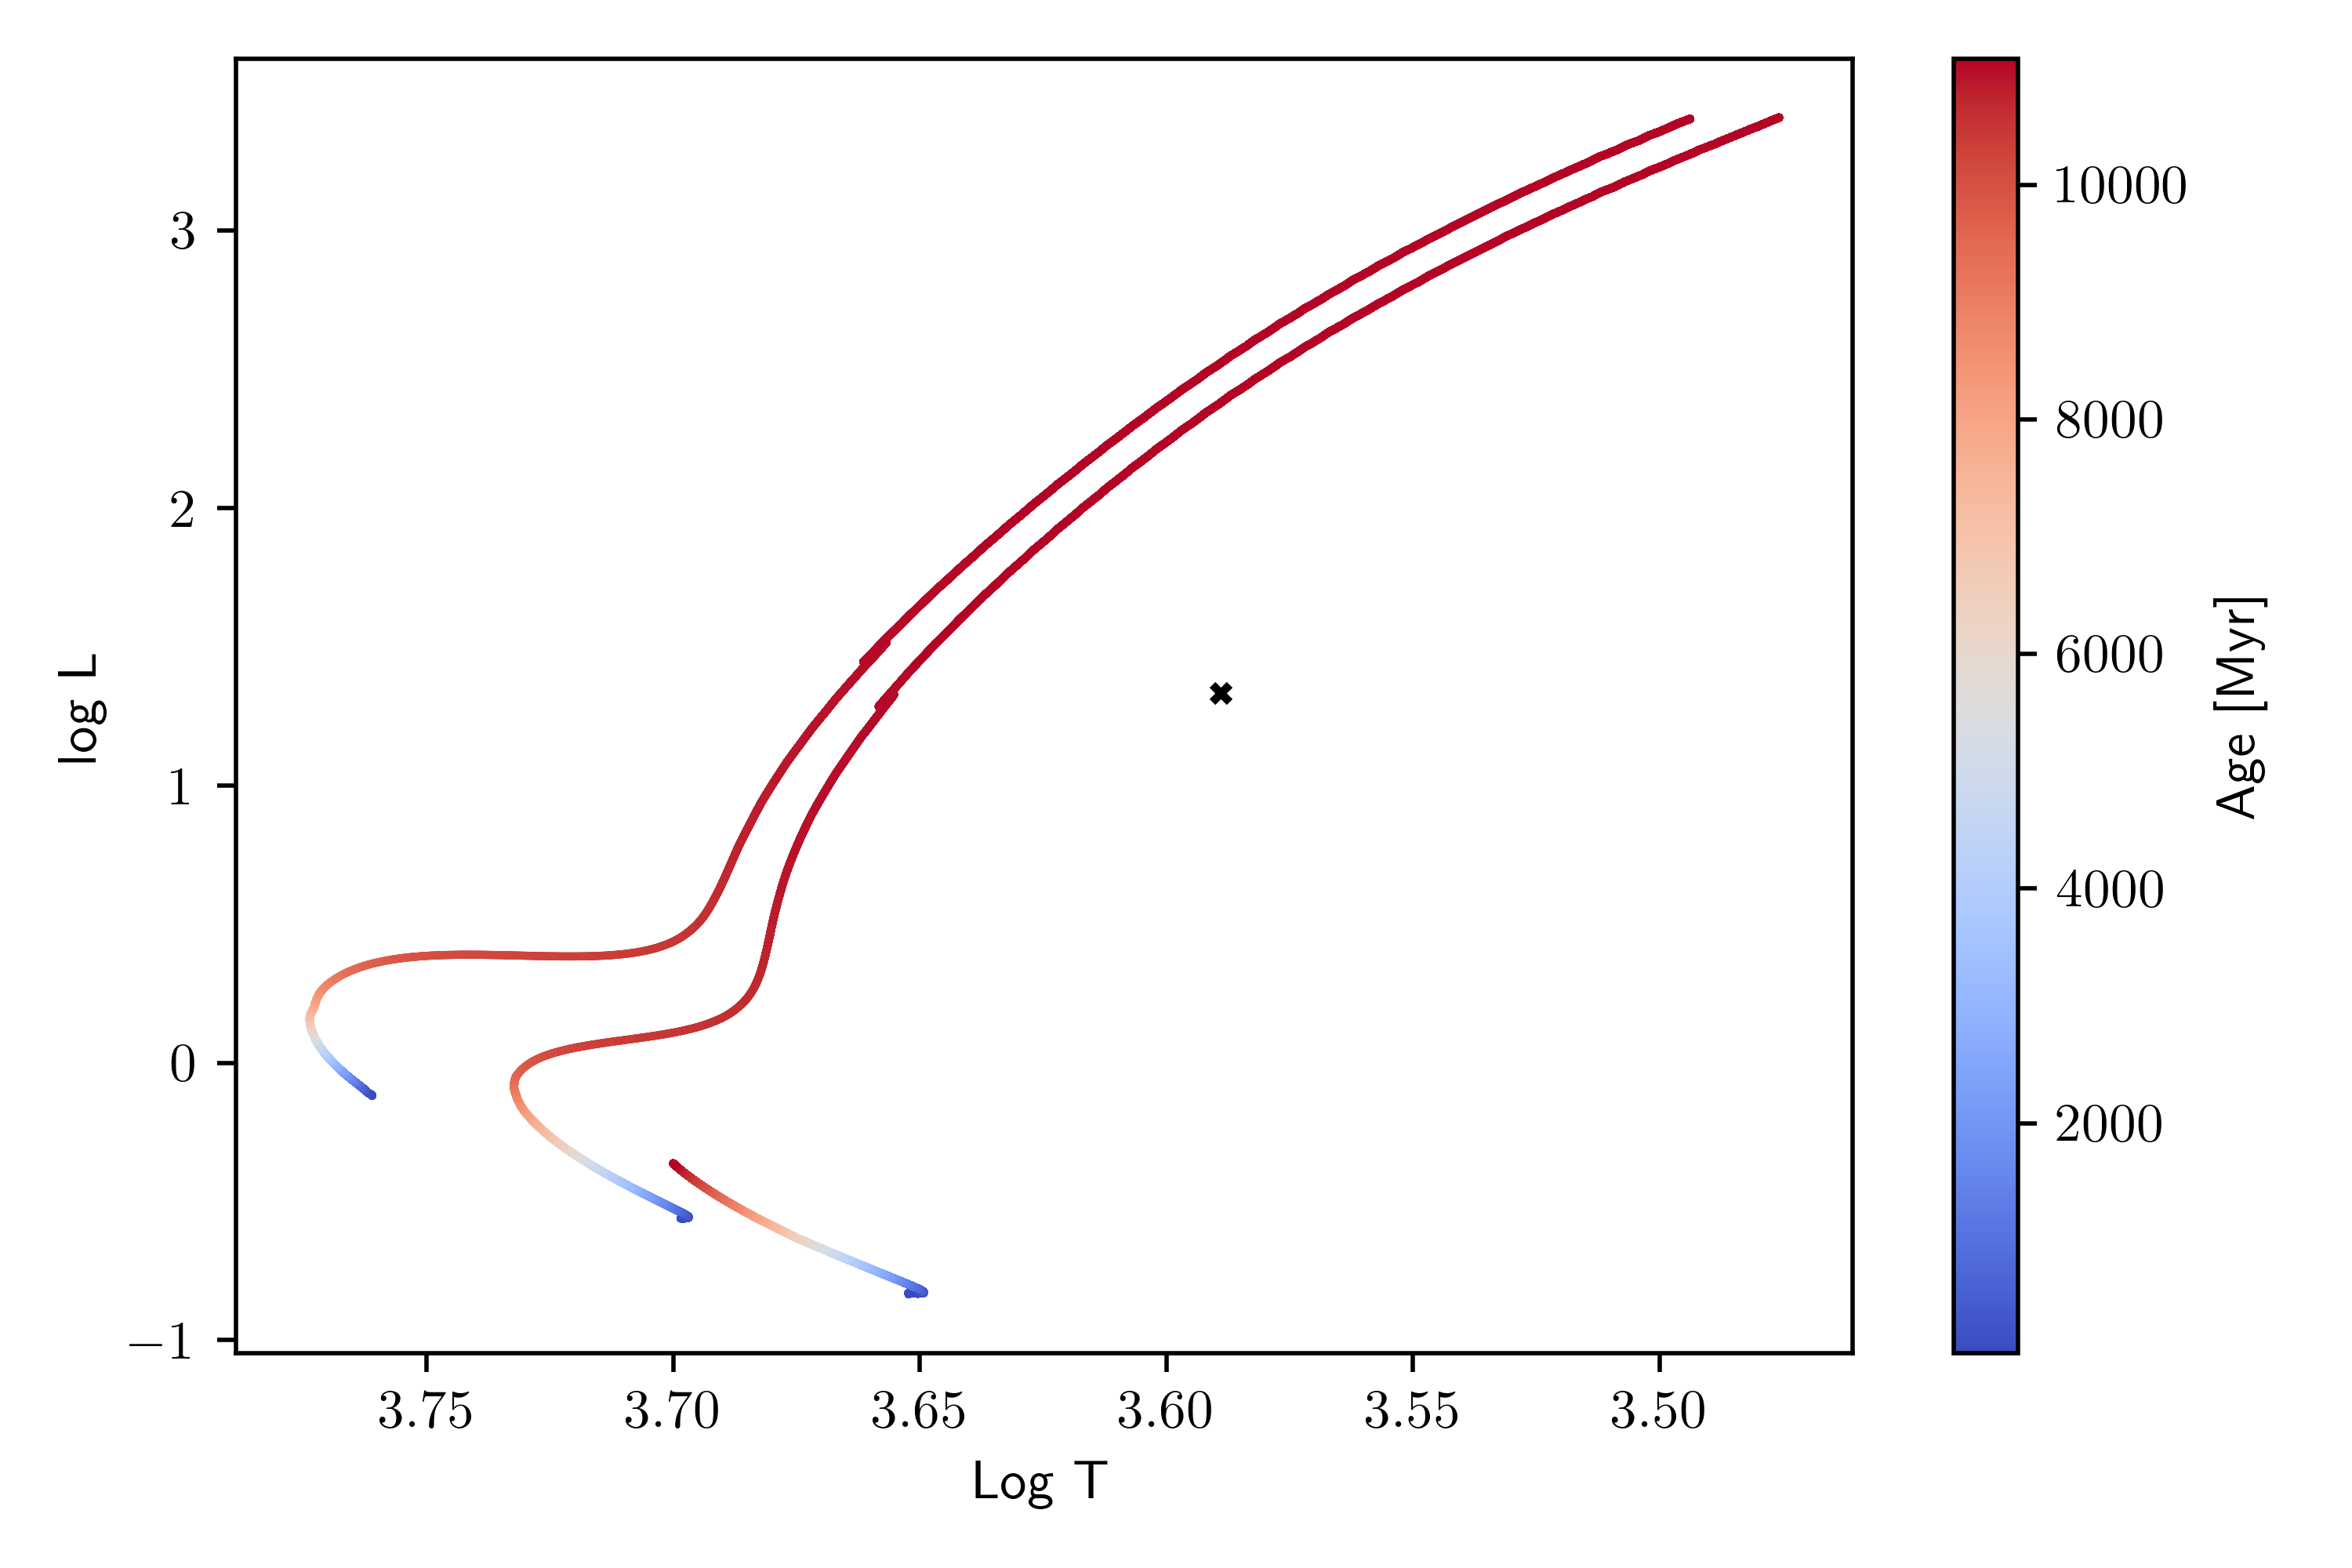
\includegraphics[scale=1]{plots/GD1070.18.22288_HR.png}
    \caption{Nearest evolutionary tracks for the cold component of GD1070.18.22288.}
    \label{HR_cold}
\end{figure}

\begin{figure}%[H]
    \centering
    \begin{subfigure}{1\textwidth}
       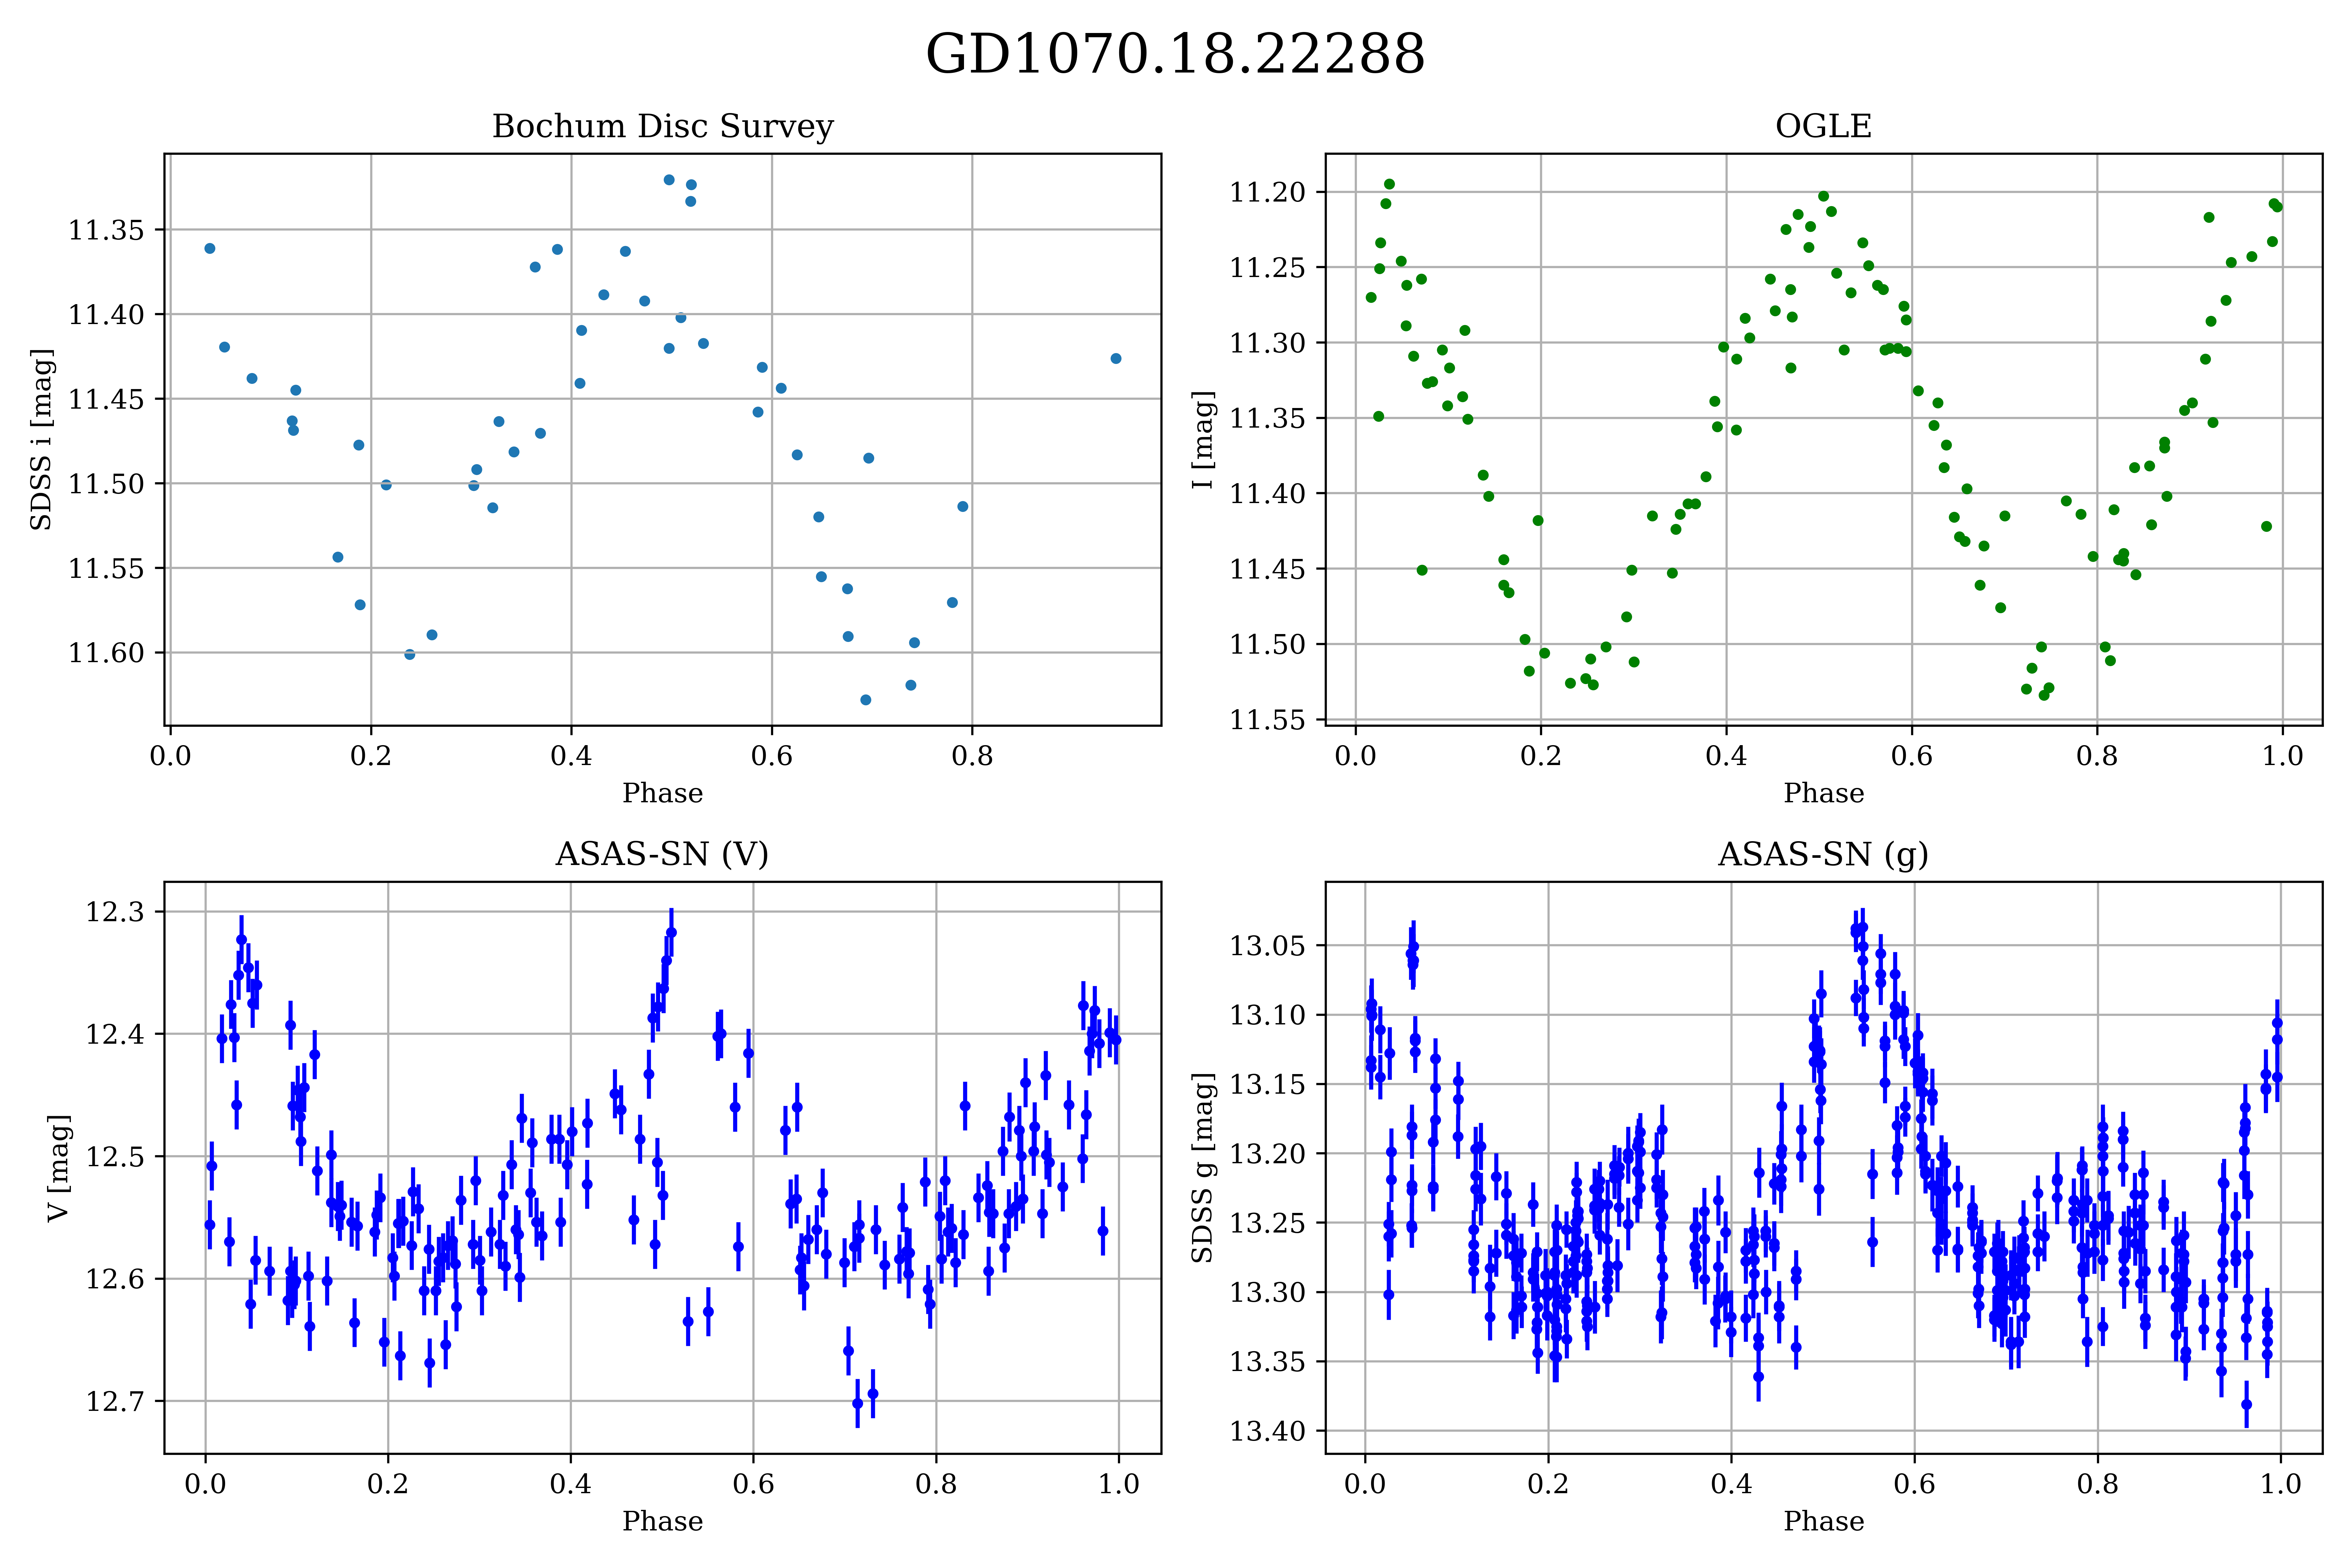
\includegraphics[width=1\linewidth]{plots/GD1070.18.22288/lc_comparsion.png}
       \caption{Light curve of GD1070.18.2288 in $4$ different bands.}\label{comp}
       \label{fig:Ng1} 
    \end{subfigure}
    
    \begin{subfigure}{1\textwidth}
       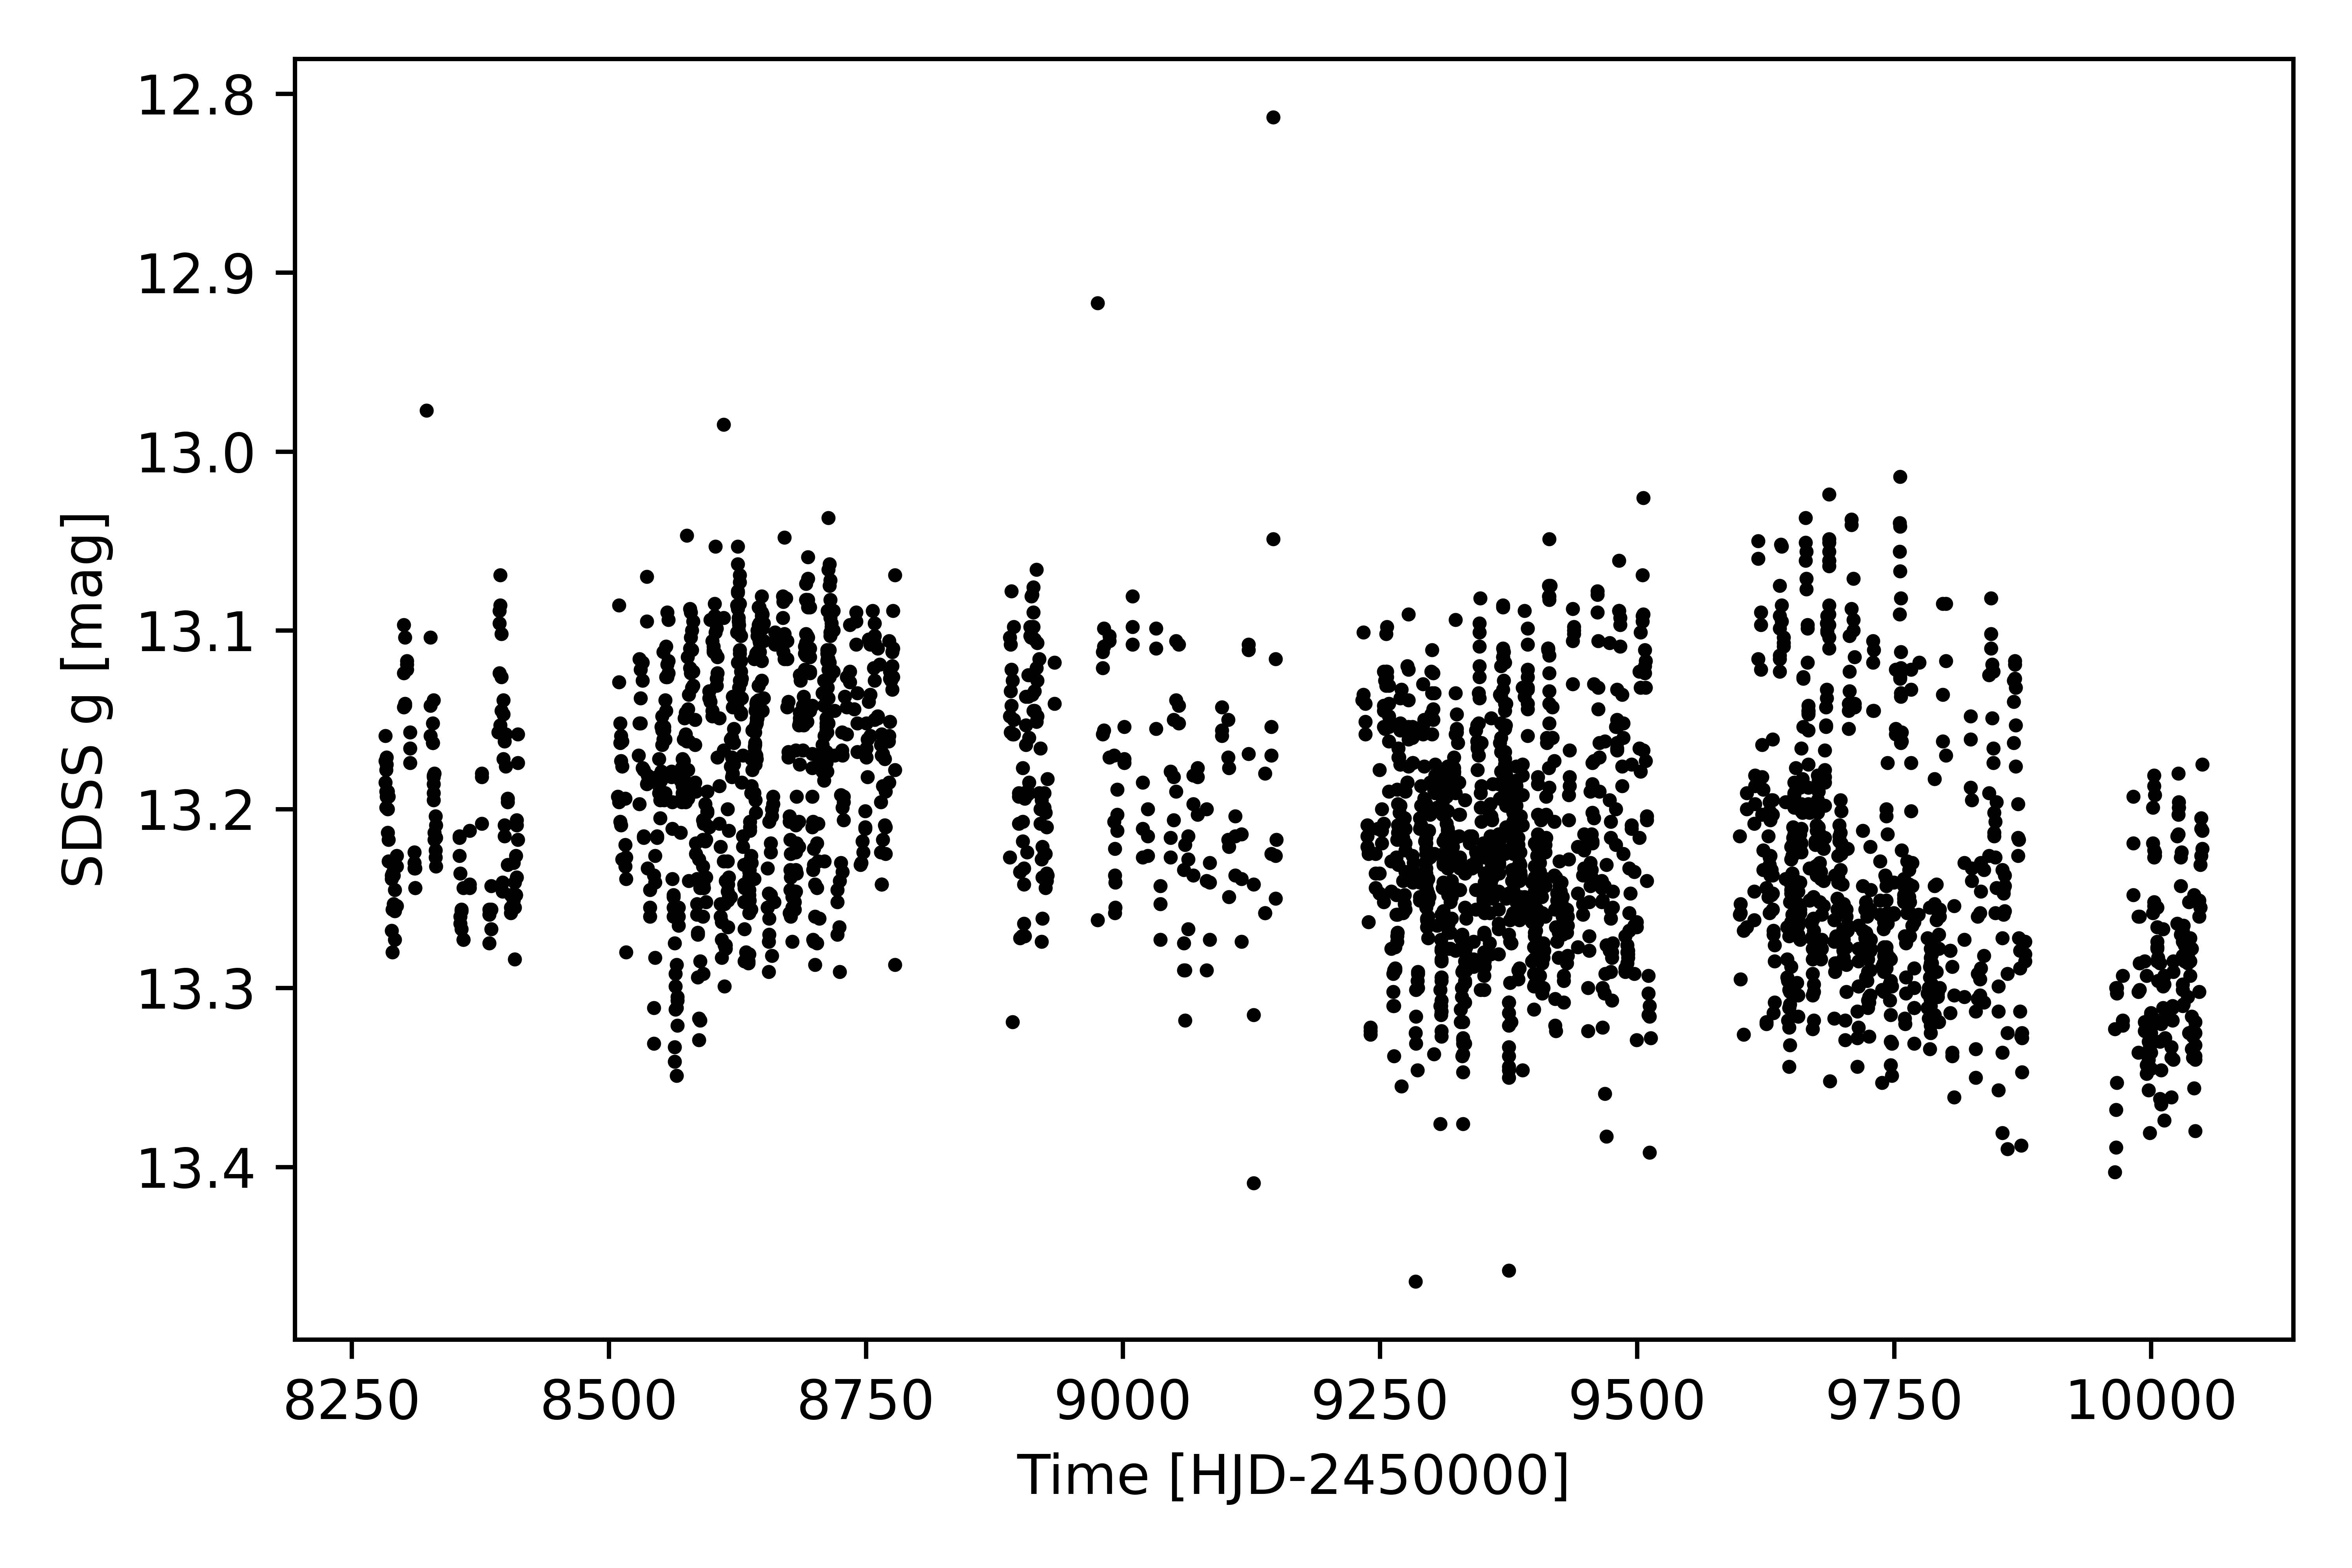
\includegraphics[width=1\linewidth]{plots/GD1070.18.22288/visibility_over_time.png}
       \caption{Change in brightness in the SDSS g band over time.}\label{evolution}
    \end{subfigure}
\end{figure}

GD1070.18.2288 was observed in the X-ray by Swift and XMM missions and published in serendipitous sources catalogues
(\citet{evans_2sxps_2020} and \citet{traulsen_xmm-newton_2020}) with id names J170801.8-410254 and J170801.8-410255
respectively. The angular distance between the position reported by the XMM DR11 catalogues \citep{traulsen_xmm-newton_2020} and the OGLE position is $105$ mas.
The positional value reported by the XMM mission is $365$ mas. The XMM object was observed few times and is transient in nature changing its flux slightly across time.
This area of the galactic disc also came to attention because of the gamma-ray source HESS J1708-410 \citep{aharonian_hess_2008} located $4.212$ arcminutes from the estimated OGLE position. 
Gamma emission from the source has an extended character, and the position reported by the OGLE falls near the $1\sigma$ region of the emission centre.
To date no plausible explanation for the origin
of the aforementioned source was found despite multiple efforts and search in various parts of the optical spectra.
One particular work \citep{van_etten_multi-wavelength_2009} observed a close vicinity of
the gamma-ray source and found emission from the point source labelled in the publication as nr $1$ (hereinafter referred to as [VFH2009] 1).
This particular point source, although quite faint, coincides with the position of GD1070.18.22280 with an accuracy of $382$ mas. 
In the publication it was found that X-ray emission is best fitted with an absorbed power law by hydrogen density $n_H=2.0\times 10^{21}$ $\textrm{cm}^{-2}$.
Interestingly, the assumed distance of $3$ kpc based on radio observations is nearly $3$ times higher than that obtained using the parallax from the Gaia DR3.
The X-ray luminosity based on the Gaia parallax for different times roughly lies in the range $L_{X}=(1-3)\cdot10^{31}$ erg/s.\hfil \break%\par\hspace{\parindent}
\hspace*{17.62482 pt} As one can see in the figure \ref{comp} there is a discrepancy between the curves in the $I$ band and the curves from ASAS-SN.
This discrepancy can be explained by investigating when light curves were collected. The OGLE
light curve is composed of observations collected from $2456467$ to $2458734$ HJD, but most samples were collected before $2457201$ HJD.
On the other hand, observations from ASAS-SN in the $g$ band were collected after $2459797$ HJD. Based on ASAS-SN archive data,
there is a visible change around $2459100$ when the period decreases from $\sim 45$ d to nearly half the value around $\sim22.4$ d.
This observation, together with the evolution of the amplitude of the variability as presented on the plot \ref{evolution},
suggests that the object represents a class of rotational variables.
This can also be partially supported by the X-ray emission from the system; it is widely known that many rotational variables like RS Canum Venaticorum can
emit X-rays with a luminosity around $\sim 10^{31}$ erg/s \citep{walter_x-rays_1980}, so the value obtained from XMM 
is consisted with emission from this type of system. It is hard to determine whether the OGLE curve exhibits changes in brightness similar to the ASAS-SN light curve,
as observations cover only a relatively short period of time. 
It is highly unlikely that the variability in the $I$ band is caused by the ellipsoidal modulation.
Tf the period would be equal to $45$ d, the inferred radii would be too small for the system to fill their Roche Lobes (unless the system would have very small total mas).
The most plausible explanation states that the system is similar to the RS Canum Venaticorum variable, undergoing mass transfer in the past.
The colder star is covered in spots that emerge due to high magnetic fields; such stars can develop a powerful coronal heating responsible for the X-ray emission.
One could investigate the X-ray spectrum of an object to find whether it is consisted with the emission from the hot plasma,
since although the object does not represent a class of ellipsoidal variables this line of investigation is dropped as it is beyond
scope of the work.% Despite lack of ellipsoidal modulation object may be interesting as it may still have greatest mass function.


\subsection{SMC720.28.40576}
\begin{figure}[H]
      \centering
      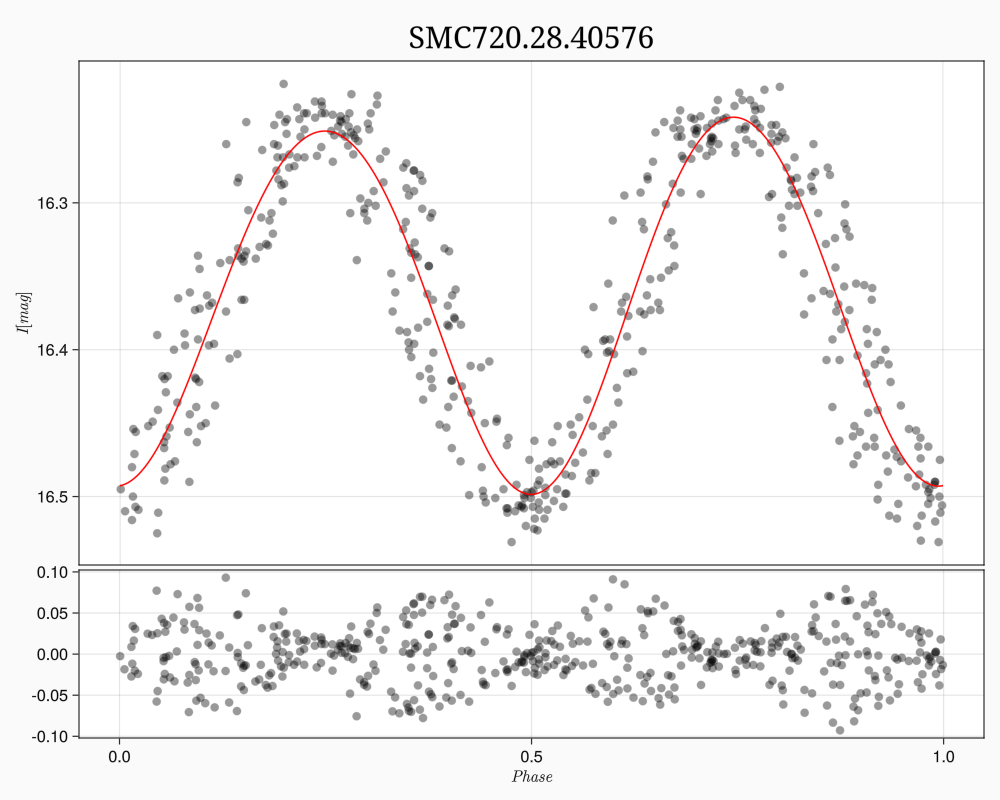
\includegraphics[scale=0.35]{plots/SMC720.28.40576_phase.png}
      \caption{Light curve of SMC720.28.40576 collected by the OGLE project.}
      \label{SMC720:lc}
\end{figure}
SMC720.28.40576 is the only object in the sample that is probably located in Magellanic Clouds as the measured parallax is statistically unsignificant.
%Estimated parameters suggest it isspectral type O according to a single-model SED fit \ref{SMC720:sed}.
The SED fit estimate suggest the star to be spectral type O, measured magnitudes with the best-fitting spectra are presented in the figure \ref{SMC720:sed}.
The estimated period of the variable is nearly half of the day; such a short period suggests a very compact setup of stars.
The PARSEC evolutionary track estimates the mass of the object to be around $16$  $\textrm{M}_{\odot}$.
Star was published already by \citep{pawlak_ogle_2016} and classified as a contact binary. Although
no companion is visible in the SED distribution, it might hide itself in the light of a primary star.
No WISE source could be found, as the nearest detection is nearly $10$ arcsec away from the position; lack of any observations
in W3 and W4 bands is very problematic as they allow to probe object in low temperatures.
%No radial velocity from Gaia is available so the mass function estimate remains unknown.
\begin{figure}[H]
    \centering
    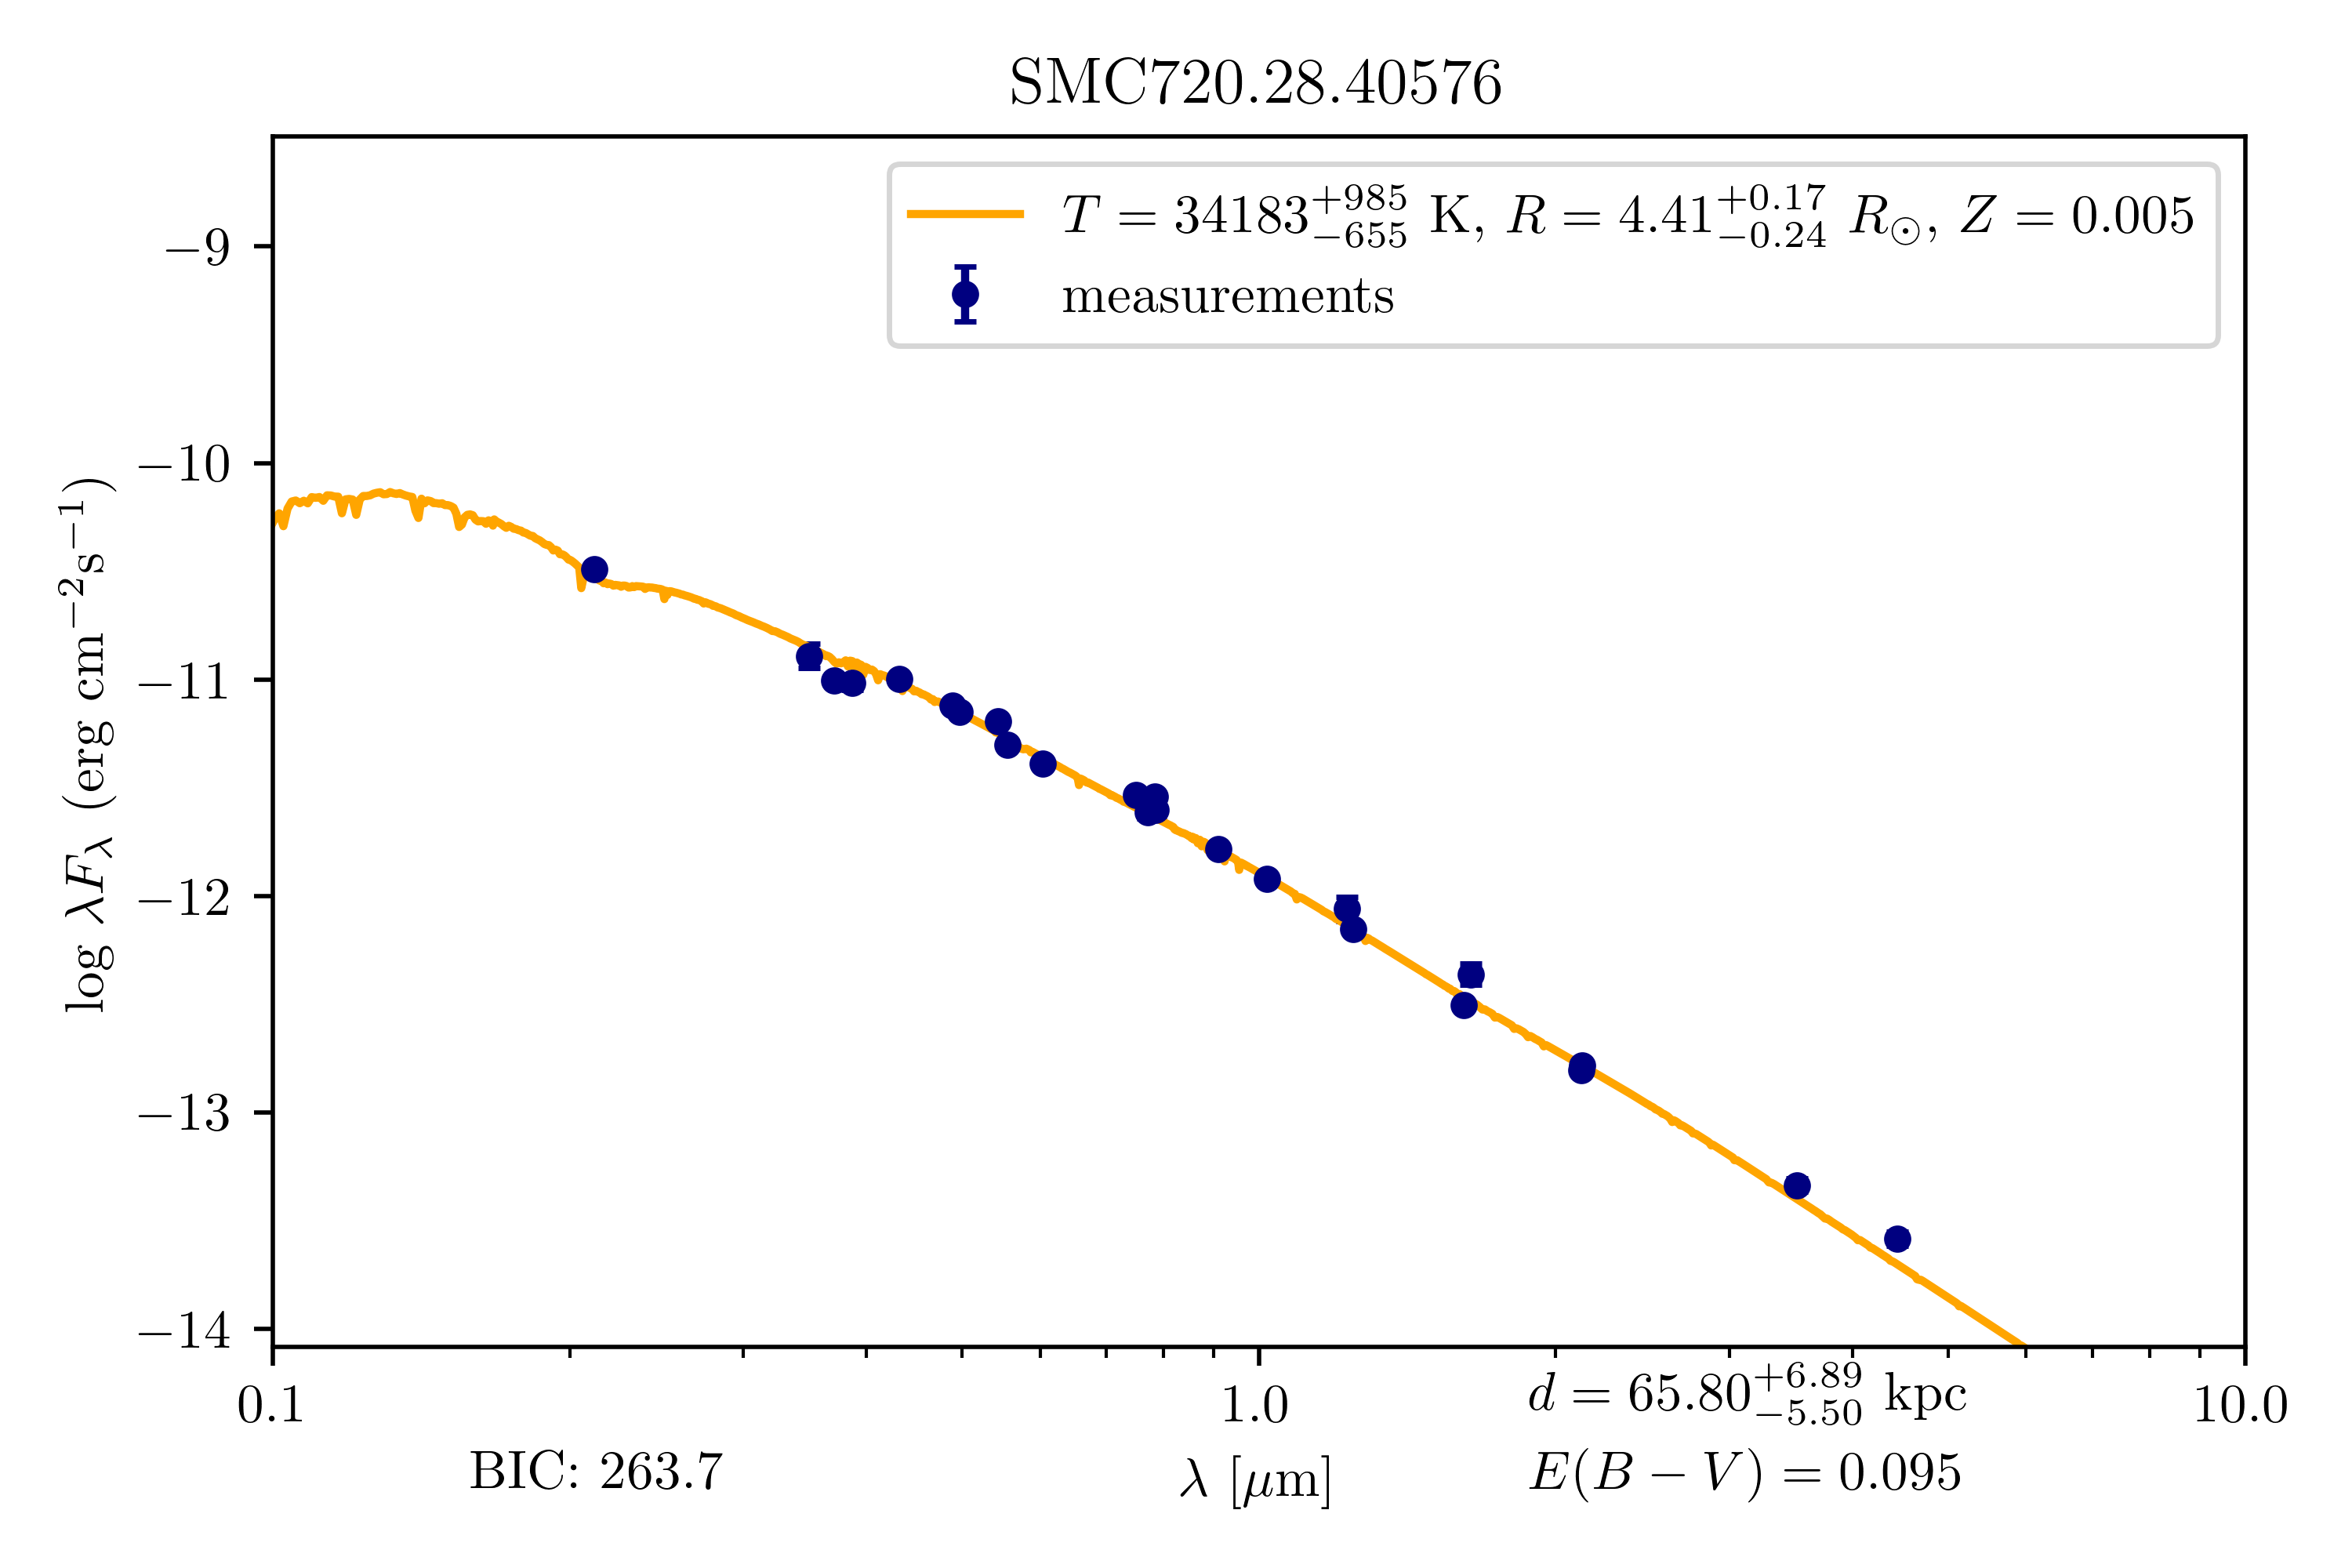
\includegraphics[scale=1]{plots/SMC720.28.40576_simple_emcee.png}
    \caption{Single model SED fit for SMC720.28.40576.}
    \label{SMC720:sed}
\end{figure}
The available data paired with the MCMC approach allow one to put some constraints on parameters of objects even if the chain had not converged. 
When the MCMC chain is not able to determine the significance of some parameters, it is reconstructing the prior distribution.
%which results in uniformly distributed region of samples.
If for some set of parameters predicted probability is very small
such region shouldn't be populated by samples, resulting in the uniformly populated region, where possible companion star can reside.
The second MCMC run was performed and $64000$ samples were drowned from the posterior distribution with $32$ walkers. 
The SED fit is performed assuming $\log g_1=4$ and $\log g_2=4$, since one expects the secondary component to be the
main sequence star. 
The results of the MCMC sampling were plotted on samples from the HYG
database\footnote{https://www.astronexus.com/hyg} and are presented in the figure \ref{posterior}
\begin{figure}[H]
    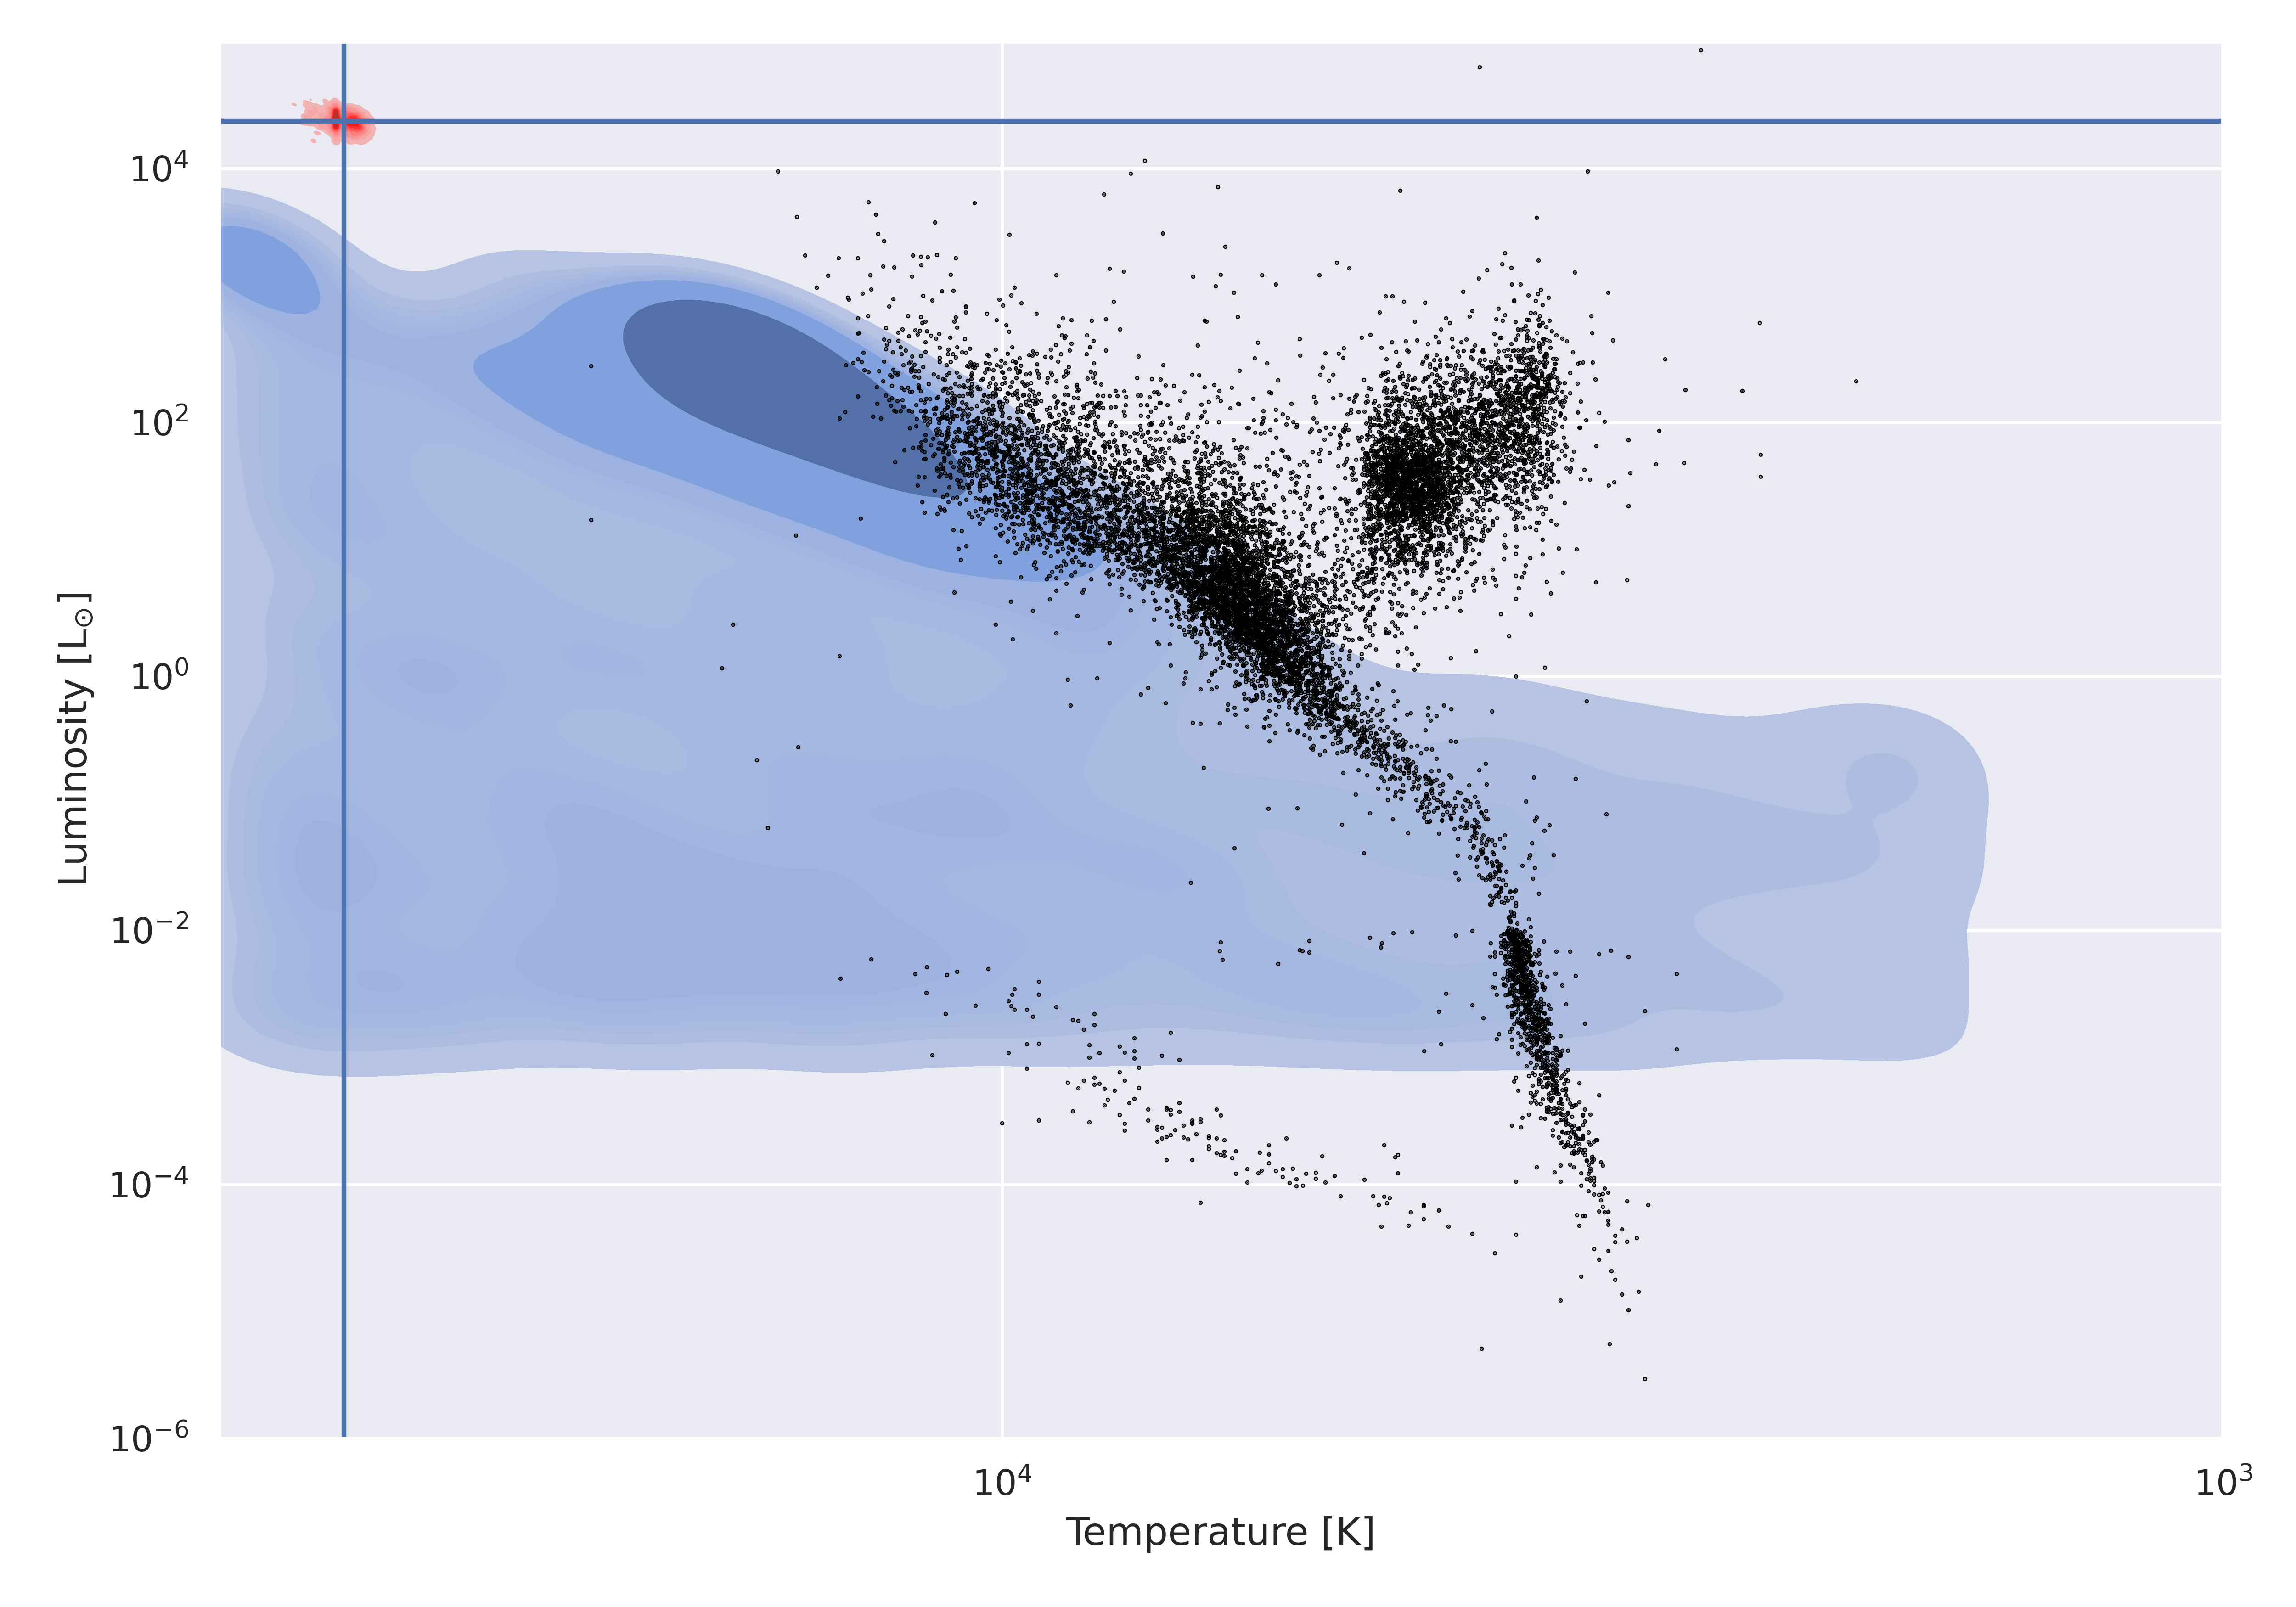
\includegraphics[scale=0.6]{plots/posterior_estimate_SMC720.png}
    \caption{The posterior estimate for the parameters of SMC720.28.40576 highlighted in red (primary component)
    and blue (secondary component).}\label{posterior}
\end{figure}
One can see that samples fill the space almost uniformly, but omit regions populated with cold and luminous stars, as those are too luminous in the infrared to reproduce observed values.
Although any object on the giant branch can be ruled out, many regions on the HR diagram can host a potential secondary companion. 
Most importantly, main sequence stars cannot be ruled out as they are to faint compared to the primary object.
%Most importantly
%few regions of main sequence stars are not excluded giving plausible candidate for secondary companion.
%Moreover it should be emphasised that in case of O type stars SED fit is quite sensitive to 
\newpage
\subsection{Remaining objects}
The majority of objects in the list can be characterised as objects with intermediate temperature. They typically have radius in order of
few solar radii and spectral type from G to A.
Although no detailed information about objects was found, two of them
are listed as nonsingle stars in the Gaia DR3 Eclipsing Binaries catalogue (BLG986.08.7, BLG931.27.36745).
The catalogue contains stars with collected light curves that matched the precomputed set of eclipsing/ellipsoidal binaries. 
Detailed processing steps can be found in the Gaia documentation \footnote[1]{https://gea.esac.esa.int/archive/documentation/GDR3/Data\_analysis/chap\_cu4nss/sec\_cu4nss\_eclipsing\_bin/}.
As part of Gaia preprocessing, the light curve is matched with the precomputed set, then the best model serves as a starting point in the local optimiser trying to refine the solution further.
The model is solved with respect to the parameters:
\begin{itemize*}
    \item fillout factors of stars $s_1$, $s_2$,
    \item inclination $i$,
    \item temperature ratio $T_1/T_2$ (effective values),
    \item argument of periastron $\omega$,
    \item time $t_0$ of eclipse.
\end{itemize*}
Both objects reported by Gaia DR3 are fitted with the contact binary model where $s_1>1$ and $s_2>1$ with almost no
temperature difference (ratio close to $1$). This result pointed out that it is possible to obtain similar results
with the contact system of two simillar stars. In such compact setup stars are in thermal equalibrium so they are able to fool the SED as
they will be well fitted with the single star model. 

This line was further investigated, and objects were fitted using the
PHOEBE simulation software (\citet*{wilson_realization_1971},\citet*{prsa_computational_2005},\citet*{conroy_physics_2020}).
The model was constructed in such a way that both stars shared the temperature $T$ (infered from a single model SED) and overflowing their Roche lobes.
Only objects from the galactic disc sample were analysed as it is possible to compare estimates of radial velocity semiamplitude with
values from the light-curve modelling.
Two masses together with the inclination $i$ and radius of the primary star $R_1$ form four parameters, which are fitted to minimise the $\chi^2$ value using the Nelder-Mead algorithm.
The second radius is no longer a free parameter, as it is controlled by a common envelope.
In the study no flux normalisation was performed, the distance and the extinction were set on the basis of the values used to perform the spectral energy distribution fit.
%What should be noted that in the SED fit mean values of luminosities were used which do not need to be equal t
The fitted values together with the $\chi^2$ values are presented in the table \ref{light_curve_fits}
together with the predicted semiamplitude of the velocity and the estimated one.
An example light curve fit for the object BLG931.27.36745 can be seen in the plot \ref{lc_plot}.

\begin{table}[H]
    \footnotesize
    \begin{center}
    \centerline{
    \begin{tabular}{lllllllll}
    Name & $M_1$ [M$_{\odot}$] & $M_2$ [M$_{\odot}$]&$R_1$ [$R_{\odot}$] &$R_2$ [$R_{\odot}$] & $i$ & $K_{\textrm{estimate}}$ [km/s] & $K_{\textrm{Gaia}}$ [km/s]&$\chi^2/dof$ \\
    \hline
    BLG931.27.36745 & $1.03$ & $0.31$ &$1.88$ & $1.21$ &$57.67^\circ$ & $50.71$ & $47.26$ & $513.67/74$ \\[0.1cm]
    GD1097.20.2300 & $1.14$ & $0.37$ & $1.56$& $1.02$ & $55.74^\circ$ &$64.05$& $75.03$ & $2929.66/118$ \\[0.1cm]
    BLG986.08.7 & $1.43$ & $0.43$& $1.82$& $1.15$ & $46.52^\circ$ & $55.17$ & $79.14$ & $827.58/72$ \\[0.1cm]
    GD2246.03.1814 & $1.09$ & $0.34$& $1.45$ & $0.92$& $50.63^\circ$ & $58.42$ & $129.93$ & $1426.90/124$\\[0.1cm]
    GD1448.27.17 & $1.58$ & $0.75$ & $2.99$& $2.16$ & $55.39^\circ$ & $69.52$ & $40.69$ & $4391.59/184$\\[0.1cm]
    \end{tabular}
    }
    \caption{Parameters used to fit the light curves of objects together with the estimates of radial velocities and the normalised $\chi^2$ values.}\label{light_curve_fits}
    \end{center}
\end{table}
Few of the light curves can be well fitted by using the contact light curve model. Objects BLG931.27.36745 or BLG986.08.7 not only
match fitted values very well but also predicted velocity semi-amplitudes are comperable to those estimated from the Gaia DR3 release. 
In some cases like GD1097.20.2300 or GD1448.27.17 there is some room for improvement; there are some discrepancies between the model
and observed curves. The most puzzling object in the whole sample is GD2246.03.1814, despite the fact that light curve modelling gave quite satisfying 
result, the predicted value of velocity semi-amplitude is twice that of the value estimated using Gaia data.
Moreover, the amplitude of radial velocity measured by the Gaia mission is equal $ 410.92 $ km/s questioning the previos estimate of radial velocity.
This can be explained either by an eccentric orbit of the star or by outliner measurements that were not removed as part of a preprocessing.
If this value is correct and if one assumes mass of the primary star from the PARSEC fit, the lower bound for the companions mass is $\sim 0.8$ M$_\odot$, detailed 
dependence between $\sin(i)$ and $M_2$ is presented in the figure \ref{second_mass}. Hence, GD2246.03.1814 is potenitally most promissing candidate for a 
dormant compact companion.

The values obtained from the fit can be quite distant from the reality, as there is not enough data to constrain the parameters of the model.
Despite this fact, as demonstrated, not only some of the objects can be well described using the contact model, but in all cases contact model can achieve an amplitude comparable to the real one. This makes such binaries one of the great weaknesses of the method described
in \citet{gomel_search_2021-2} as a simple contact binary can easily be classified as a potential candidate.
 
%\begin{figure}
%    \centering
%    \includegraphics[scale=0.6]{plots/modeling_phoebe_contact_BLG931.27.36745.jpg}
%    \caption{The light curve fit with the contact binary model for BLG931.27.36745.}\label{lc_plot}
%\end{figure}
%\begin{figure}
%    \centering
%    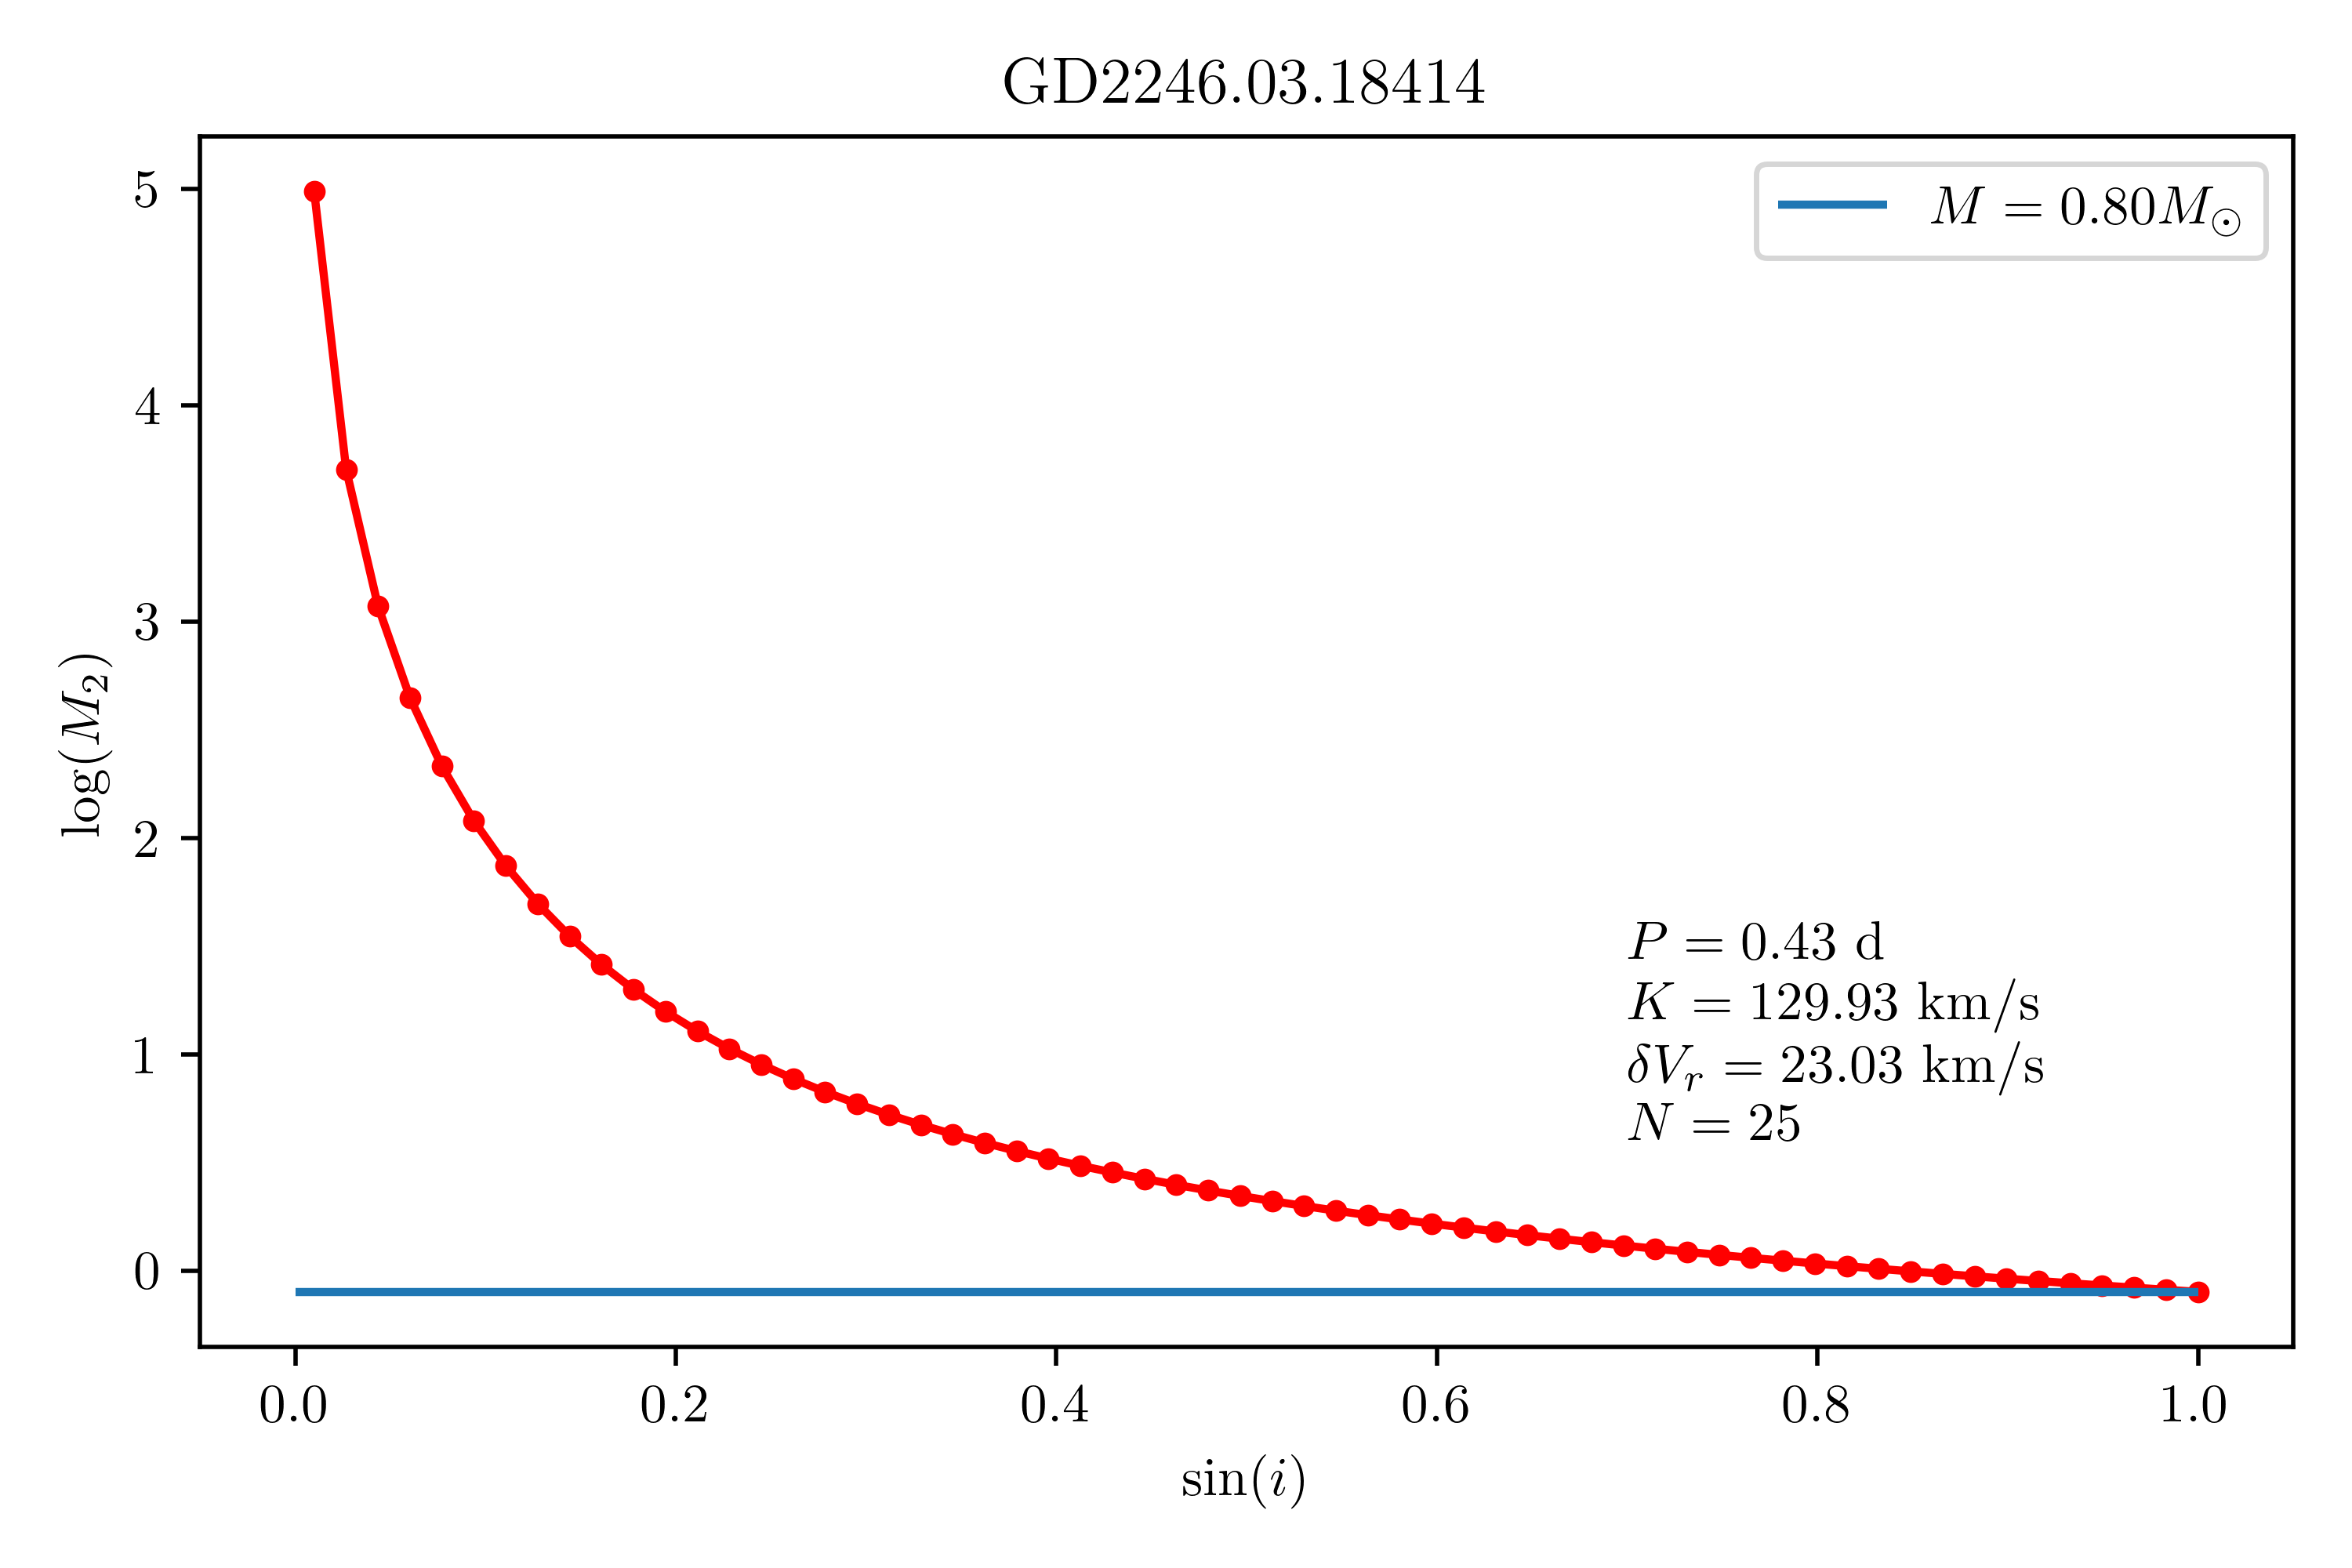
\includegraphics[width=\textwidth]{plots/GD2246.03.18414second_mass.png}
%    \caption{The light curve fit with the contact binary model for BLG931.27.36745.}\label{second_mass}
%\end{figure}
\begin{figure}
    \begin{subfigure}{1\textwidth}
        \centering
        \includegraphics[scale=0.6]{plots/modeling_phoebe_contact_BLG931.27.36745.jpg}
        \caption{The light curve fit with the contact binary model for BLG931.27.36745.}\label{lc_plot}
    \end{subfigure}
    
    \begin{subfigure}{1\textwidth}
        \centering
        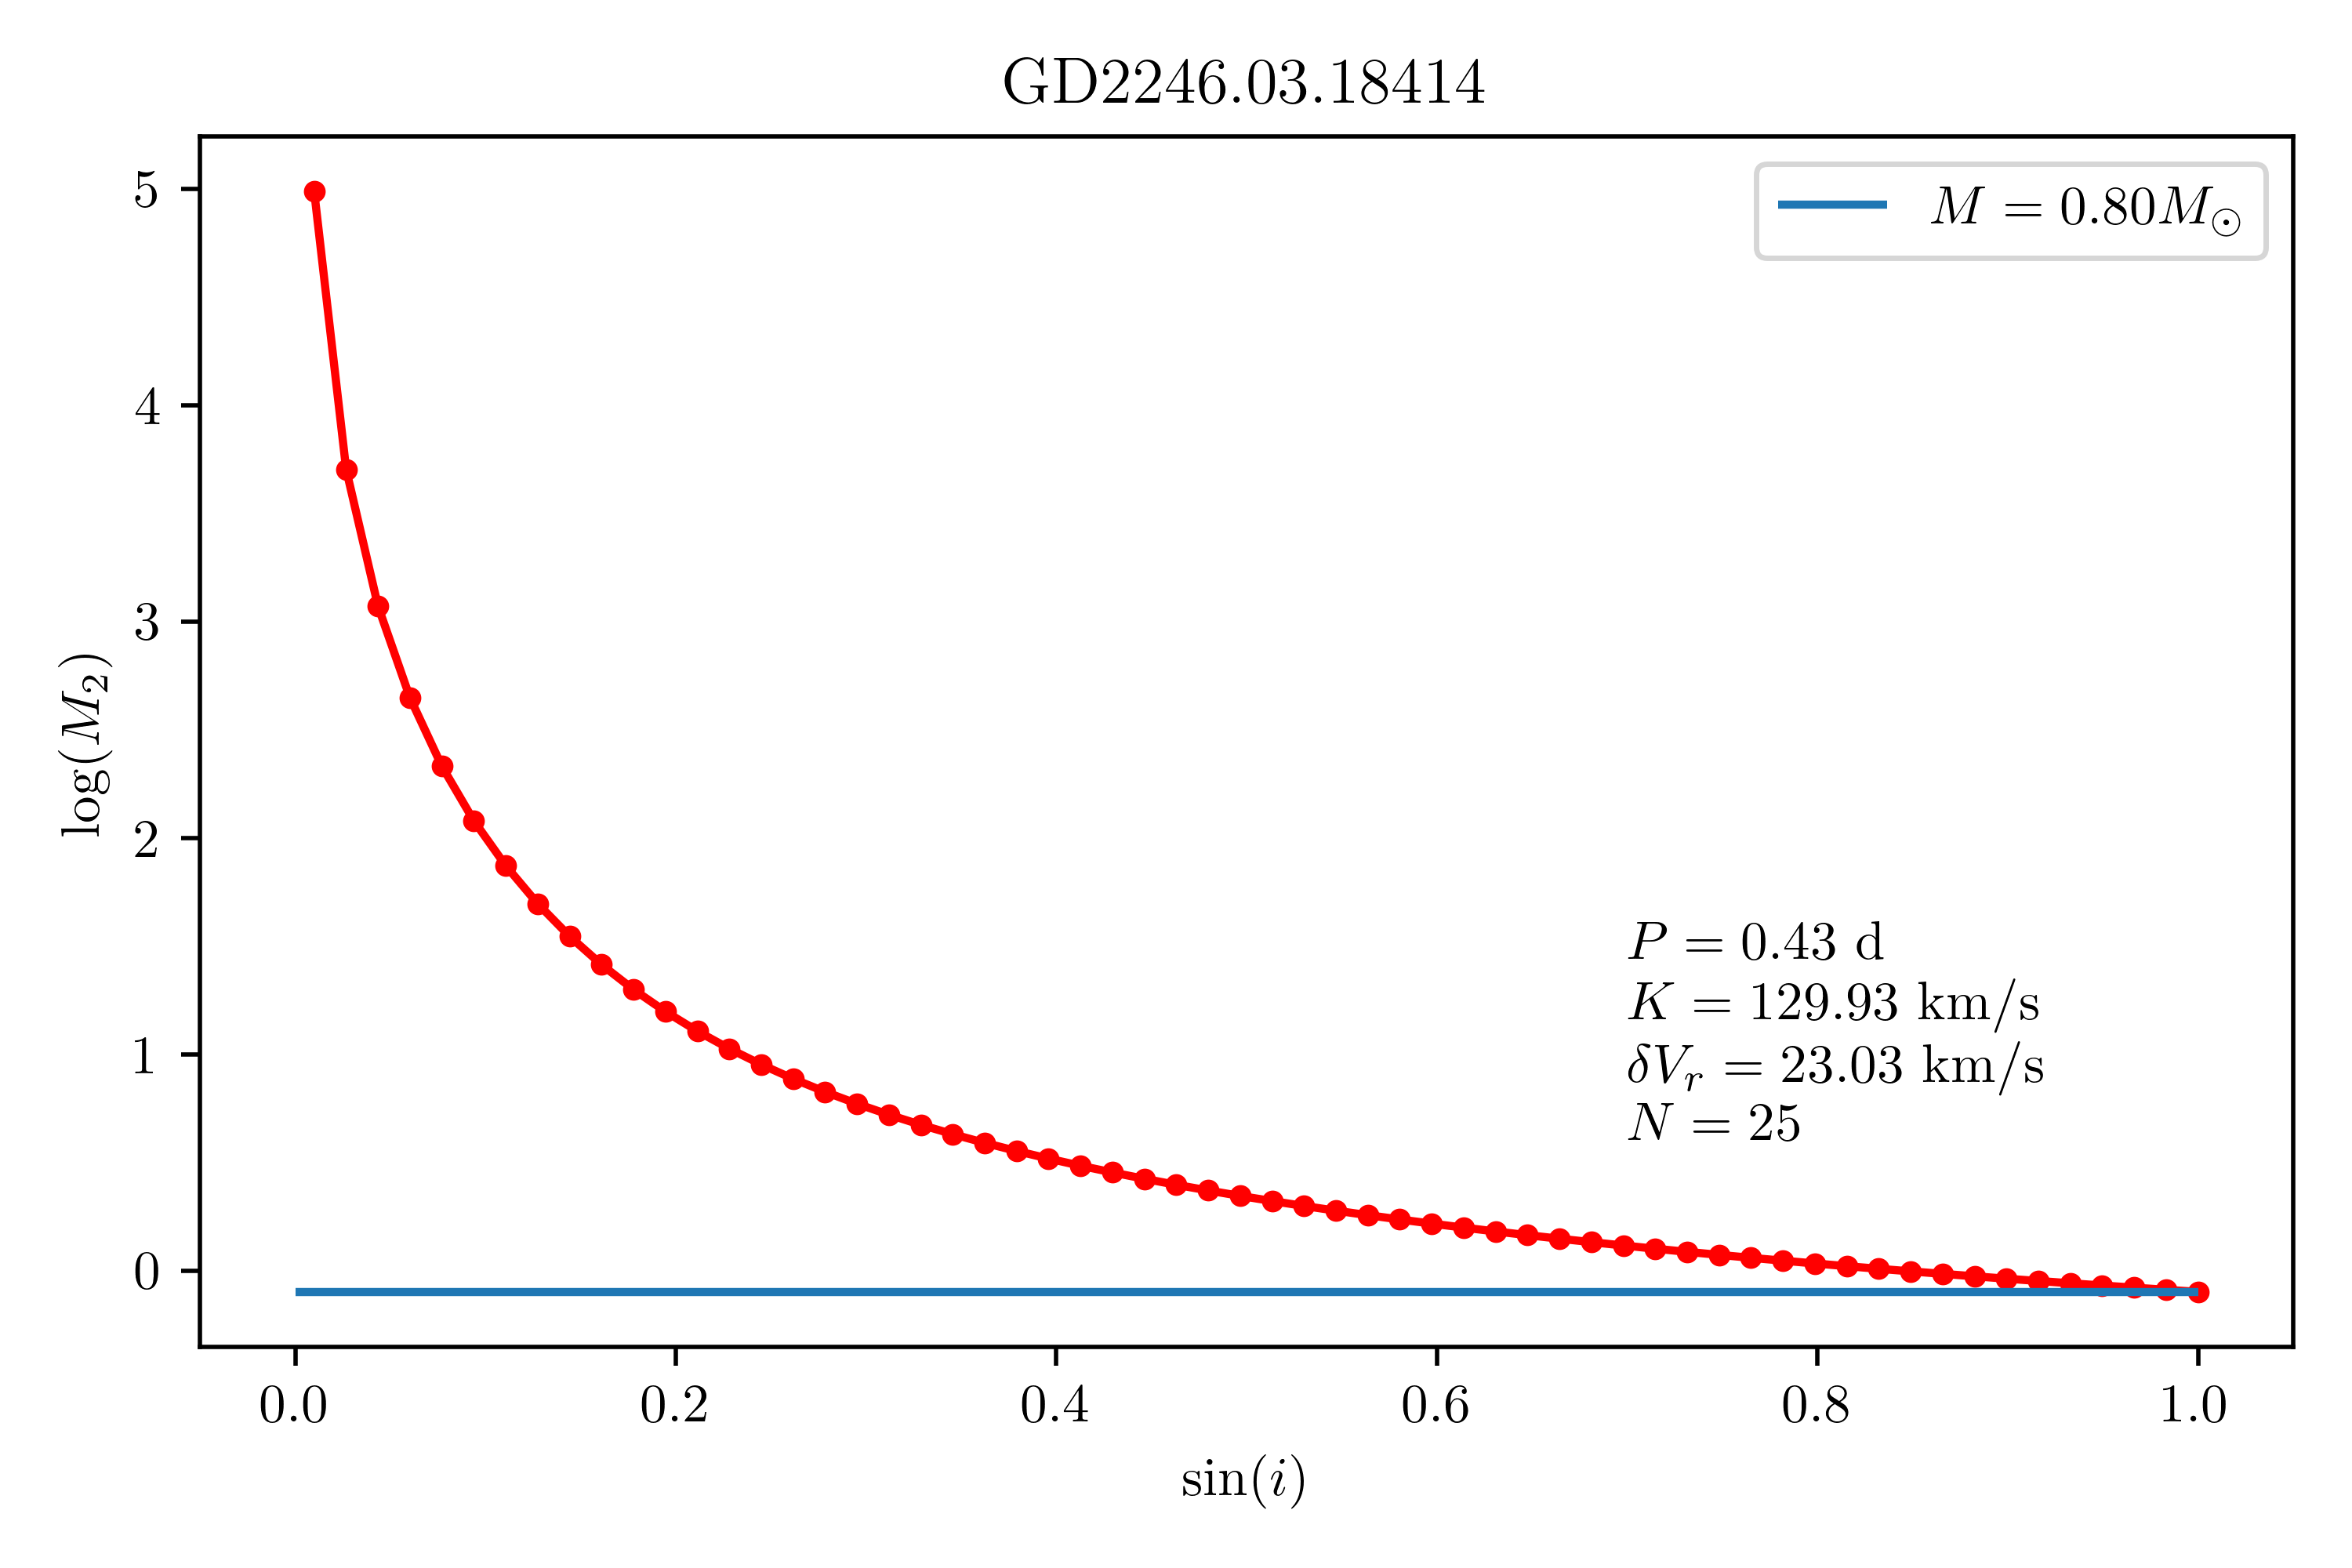
\includegraphics[width=\textwidth]{plots/GD2246.03.18414second_mass.png}
        \caption{Dependence between the companion mass and the binary inclination for GD2246.03.1814.}\label{second_mass}
    \end{subfigure}
\end{figure}


\chapter{Discussion \& Conclusions}

Of the total $8515$ objects investigated in this study, only 14 were classified as plausible candidates for compact companion binaries.
Further investigation into the sample revealed one rotational variable and suggested an alternative explanation for tweelve objects in the form of
contact binaries with an intermediate mass ratio. It is impossible to pinpoint exact nature of objects as only spectroscopic observations allow to determine 
radial velocitie of stars and true nature of companion objects. All of those candidates can potentially host neutron stars/black holes, but
due to great amounts of contact binaries in the universe probability contact sceniario seem to be much more plausible.
Gaia DR3 semiamplitude estimations suggest most of the companions are not compact at all, even for stars with the estimated radial velocity amplitude $\sim100$ km/s of the secondary companion being too low for compact star. 
Only one object distinguishes itself from the rest with the high estimate of the velocity semiamplitude $\approx120$ km/s, which is difficult to explain with a simple contact binary model. 
Based on the PARSEC estimate, a lower bound for companion mass is equal $\approx0.8$ M$_{\odot}$ making the candidate quite promissing. 

Until now, only one publication tried to perform any kind of follow-up observations of candidates described in \citet{gomel_gaia_2022} (also 
found with the method described in \citet{gomel_search_2021-2}). \citet{nagarajan_spectroscopic_2023} selected sample of objects that were promissing
and obtained epoche radial velocities for them. It was found that all selected objects cannot host any type of compact object as velocity semiamplitudes are too low.
It was suggested that such varaibles can be easily explained by contact binaries with or without spots. This conclusion is similar in some sense to the results presented in this work.
Such an explanation is quite convincing as such objects should be quite common contrary to the black hole binaries. It was pointed out that stars with the nearly overflowing
primary star should be rather rare as this phase of a binary evolution is very shortlived. Hence system should be either well-detached or overflowing its Roche lobe,
resulting in an X-ray binary.  In fact in \citet{gomel_search_2021-2} the method presented was applied to some X-ray binaries with black hole companions and
found that at least some of them would be detected.
As it was noted in the introduction, creation of such systems is rather rare so potential sample of black holes that can be revealed seem
to be small compared to black holes in wider binaries.
Moreover, as demonstrated a simple contact model can be easily classified as a candidate. 
Therefore, the potential sample can be primarily populated by those common false-positive contaminants.
Although \citet{nagarajan_spectroscopic_2023} did not find any compact companion,
more objects should be investigated to better characterise the population of those high-amplitude binaries.

\bibliography{Bachelor} 
\bibliographystyle{mnras}
\begin{appendices}
    \chapter{Light curve \& SED plots}
    \summary{BLG986.08.7}
    \summary{GD2246.03.18414}
    \summary{GD1097.20.23000}
    \summary{GD1448.27.17}
    \summary{BLG931.27.36745}
    \summary{LMC574.11.3407}
    \summary{LMC606.30.48}
    \summary{LMC751.15.2886}
    \summary{MBR108.18.3}
    \summary{MBR236.09.433}
    \summary{SMC711.22.1068}
    \summary{SMC720.28.40576}
    \summary{SMC742.26.330}
    %\restoregeometry
    \chapter{Semiamplitude estimate from Gaia DR3}
    Let's now assume, that a radial velocity can be factored into two separate movements: the centre of mass movement (with velocity $v_0$) and the 
    circular motion with semiamplitude $K$. Under following 
    assumptions one can find, that samples of radial velocity can be written as 
    \begin{equation}
        V_i=v_0+K\cos{(2\pi X_i)}
    \end{equation}
    where $X_i$ is a sample from $\mathcal{U}(0,1)$. This allows to simplify the variance estimator as  
    \begin{equation}
        \sigma^2=\frac{1}{n}\sum_i (\overline{V}-V_i)^2\approx \frac{K^2}{N}\sum \cos^2{(2\pi X_i)}=\frac{K^2}{N}\sum_i \frac{\cos{(4\pi X_i)}+1}{2}
    \end{equation}
    where the simplification $\overline{V}\approx v_0$ is used. Now, one would like to obtain some statistical properties of this variance estimator such as the expected value.
    One can clearly check, that $\mathbb{E}\cos{(4\pi X_i)}=0$. Hence 
    \begin{align}\label{semi}
        \mathbb{E} \sigma^2 = \frac{K^2}{2N}\cdot N = \frac{K^2}{2}.
    \end{align}

    \chapter{Light curve modeling}
    \begin{figure}[H]
        \centering
        \begin{adjustwidth}{-0.5in}{-0.5in}
        \begin{subfigure}{0.6\textwidth}
            \centering
            \includegraphics[width=1\textwidth]{plots/modeling_phoebe_contact_BLG931.27.36745.jpg}
            \caption{PHOEBE lightcurve fit for BLG931.27.36745. }
        \end{subfigure}
        %\hfill
        \begin{subfigure}{0.6\textwidth}
            \centering
            \includegraphics[width=1\textwidth]{plots/modeling_phoebe_contact_BLG986.08.7.jpg}
            \caption{PHOEBE light curve fit for BLG986.08.7. }
        \end{subfigure}
        \end{adjustwidth}
   \end{figure}
    \begin{figure}[H]
        \centering
        \begin{adjustwidth}{-0.5in}{-0.5in}
        \begin{subfigure}{0.6\textwidth}
            \centering
            \includegraphics[width=1\textwidth]{plots/modeling_phoebe_contact_GD1448.27.17.jpg}
            \caption{PHOEBE light curve fit for GD1448.27.17.}
        \end{subfigure}
        %\hfill
        \begin{subfigure}{0.6\textwidth}
            \centering
            \includegraphics[width=1\textwidth]{plots/modeling_phoebe_contact_GD1097.20.23000.jpg}
            \caption{PHOEBE light curve fit for GD1097.20.23000. }
        \end{subfigure}
        \end{adjustwidth}
   \end{figure}
   \begin{figure}[H]
    \centering
    \includegraphics[width=\textwidth]{plots/modeling_phoebe_contact_GD2246.03.18414.jpg}
    \caption{PHOEBE light curve fit for GD2246.03.18414. }
    \end{figure}
\end{appendices}
\end{document}